As mentioned in Chapter~\ref{ch:introduction}, swarm behaviors are emergent behaviors that arise from the interactions of a number of simple individuals in a group~\cite{Camazine2001}. Researchers in artificial intelligence and swarm robotics use simulated agents or physical robots to mimic and understand the swarm behaviors observed in nature, such as foraging, aggregation, and flocking. This approach is what we refer to as understanding from synthesis. It has been used to validate models of swarm behaviors, provide insights, or even generate new hypotheses~\cite{J.Halloy2007}. The design of controllers for the simulated agents or physical robots usually adheres to similar conditions to those found in biological swarm systems.
For example, the controllers are distributed, that is, there is no central control for the swarm; the structure of the controllers is relatively simple.

In this chapter, we demonstrate how the proposed system identification (coevolutionary) method allows a machine to infer the behavioral rules of a group of homogeneous agents in an autonomous manner. A replica, which resembles the agents under investigation in terms of behavioral capabilities, is mixed into the group. The coevolutionary algorithm consists of two competitive populations: one of \textit{models}, to be executed on the replica, and the other of \textit{classifiers}. The classifiers observe the motion of an individual\footnote{Note that `individual/robot' in the context of swarm behaviors refers to a single unit. It could refer to an agent under investigation or a replica executing a model. However, in the context of evolutionary algorithms (see Section~\ref{sec:optimization_algorithm_swarm}), `individual' refers to a chromosome.} in the swarm for a fixed time interval. They are not, however, provided with the individual's sensory information. Based on the individual's motion data, a classifier outputs a Boolean value indicating whether the individual is believed to be an agent or replica. The classifier gets a reward if and only if it makes the correct judgment. The fitness of the classifiers thus depends solely on their ability to discriminate between the agents and the replica. Conversely, the fitness of the models depends solely on their ability to `trick' the classifiers into categorizing them as an agent. Consequently, our method does not rely on predefined metrics for measuring the similarity of behavior between models and agents; rather, the metrics (classifiers) are produced automatically in the learning process. Our method is inspired by the Turing test~\cite{Turing1950, Harnad2000}, which machines can pass if behaving indistinguishably from humans. Similarly, the models, which evolve, can pass the tests by the coevolving classifiers if behaving indistinguishably from the agents. We hence call our method~\textit{Turing Learning}.

To validate the~\textit{Turing Learning} method, we present two case studies on canonical problems in swarm robotics: self-organized aggregation~\cite{Gauci2014_ijrr} and object clustering~\cite{Melvin2014_aamas}. We show that observing individual motion is sufficient to guide the learning of these collective behaviors. In this chapter, we only present the simulation results. A real-world validation using physical robots based on one of the case studies will be presented in Chapter~\ref{ch:swarm_physical_implementation}.

%This chapter is organized as follows. Section~\ref{sec:methodology_swarm_simulation} describes the implementation of~\textit{Turing Learning} (Section~\ref{sec:turing_learning_swarm_simulation}) and the two swarm behaviors (Section~\ref{sec:case_studies_swarm_simulation}) investigated in this chapter. Section~\ref{sec:simulation_platform_setups} introduces the simulation platform (Section~\ref{sec:platform_swarm_simulation}) and simulation setups (Section~\ref{sec:setup_swarm_simulation}) for performing coevolution runs. Section~\ref{sec:results_swarm_simulation} presents the results obtained from the two case studies. Section~\ref{sec:analysis_evolved_models_swarm_simulation} analyzes the evolved models from the perspective of both local behaviors and global behaviors. Section~\ref{sec:coevolutionary_dynamics_simulation_swarm_simulation} investigates the coevolutionary dynamics. Section~\ref{sec:analysis_evolved_classifiers_swarm_simulation} systematically investigates the evolution of classifiers, showing how to construct a robust classifier system to potentially detect abnormal behaviors in the swarm. Section~\ref{sec:observing_a_subset_agents_swarm_simulation} presents the results of only observing a subset of agents in the swarm. Section~\ref{sec:evolving_control_and_morphology_swarm_simulation} presents a study where an aspect of the agents' morphology (their field of view) and brain (controller) are inferred simultaneously. Section~\ref{sec:evolving_other_behaviors_swarm_simulation} shows the results of inferring other behaviors. Section~\ref{sec:noise_study_swarm_simulation} presents a noise study. Section~\ref{sec:summary_simulation_swarm} summaries the findings in this chapter.

This chapter is organized as follows. Section~\ref{sec:methodology_swarm_simulation} describes the implementation of~\textit{Turing Learning} and the two swarm behaviors under investigation. Section~\ref{sec:simulation_platform_setups} introduces the simulation platform and setups for performing coevolution runs. Section~\ref{sec:results_swarm_simulation} presents the results obtained from the two case studies. In particular, Section~\ref{sec:analysis_evolved_models_swarm_simulation} analyzes the evolution of models, objectively measuring their quality in terms of local and global behaviors. Section~\ref{sec:coevolutionary_dynamics_simulation_swarm_simulation} investigates the coevolutionary dynamics. Section~\ref{sec:analysis_evolved_classifiers_swarm_simulation} investigates the evolution of classifiers, showing how to construct a robust classifier system to potentially detect abnormal behaviors in the swarm. Section~\ref{sec:observing_a_subset_agents_swarm_simulation} studies the effect of observing only a subset of agents in the swarm. Section~\ref{sec:evolving_control_and_morphology_swarm_simulation} presents a study where an aspect of the agents' morphology (their field of view) and brain (controller) are inferred simultaneously. Section~\ref{sec:evolving_other_behaviors_swarm_simulation} shows the results of using~\textit{Turing Learning} to learn other swarm behaviors. Section~\ref{sec:noise_study_swarm_simulation} presents a study showing the method's sensitivity to noise. Section~\ref{sec:summary_simulation_swarm} summaries the findings in this chapter.


\section{Methodology}\label{sec:methodology_swarm_simulation}

In this section, we present the~\textit{Turing Learning} method and two case studies: self-organized aggregation~\cite{Gauci2014_ijrr} and object clustering~\cite{Melvin2014_aamas}. In both case studies, individuals execute simple behavioral rules that lead to meaningful emergent behaviors on a global level. 

\subsection{Turing Learning}\label{sec:turing_learning_swarm_simulation}

\textit{Turing Learning} uses a coevolutionary algorithm that comprises two populations: one of models, and one of classifiers. These populations coevolve competitively. In the following, we describe the models, classifiers, optimization algorithm, fitness calculation method and termination criterion. 

\subsubsection{Models} 

We assume to have a replica that has actuation and sensing abilities that are equivalent to those of the agents under investigation. In other words, the replica must be able to produce behavior that---to an external observer (classifier)---is indistinguishable to that of the agent. For example, if the observer tracks the position of a bird in three dimensions (3D), the replica (which could be artificial or real) must be able to produce 3D motion data. There can be one or more replicas. In Chapters~\ref{ch:swarm_simulation} and~\ref{ch:swarm_physical_implementation},  the replica(s) will be mixed into a group of homogeneous agents. They should therefore be perceived by the agents as con-specifics~\cite{J.Halloy2007}. In Chapter~\ref{ch:interaction}, a single replica is studied in isolation.

Models are executed on replicas. The models can be represented explicitly (e.g., parameters) or implicitly (e.g., artificial neural networks). %In principle, multiple replicas can be inserted to assess multiple models simultaneously. 

\begin{figure}[!t]
	\centering
	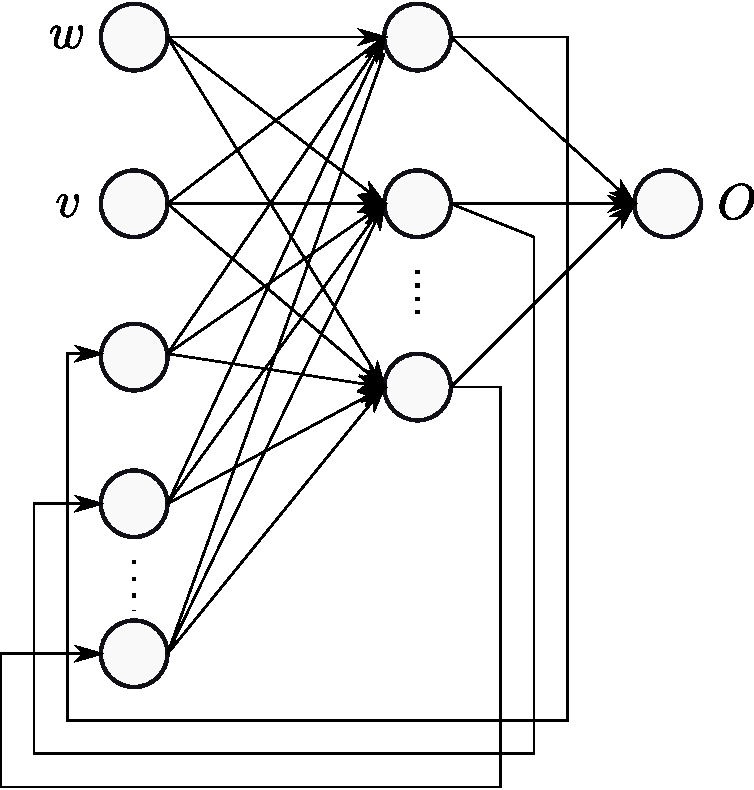
\includegraphics[width=3.0 in]{Neural_Network_CF_Swarm.pdf}
	\caption{The plot shows the structure of a classifier, which is a recurrent Elman neural 
    network, with $i$ inputs, $h$ hidden neurons, and one output neuron ($O$). $O$ is used for making a judgment. Two bias neurons (which are not shown) with a constant input of 1.0 are connected to each neuron of the hidden and output layers. See text for details.}
	\label{fig:neural_network_cf_swarm}
\end{figure}

\subsubsection{Classifiers}

The classifier can be any algorithm that takes a sequence of data about the observed individual as input, and outputs a decision (i.e., whether the observed individual is believed to be an agent or replica). 

We represent the classifier as a recurrent Elman neural network~\cite{Elman1990}, which is shown in Figure~\ref{fig:neural_network_cf_swarm}. The network has $i$ inputs, $h$ hidden neurons and one output neuron. Each neuron of the hidden and output layers has a bias. The network has a total of $(i+1) h + h^2 + (h+1)$ parameters, which all assume values in $\mathbb{R}$. The activation function used in the hidden and the output neurons is the logistic sigmoid function, which has the range $\left(0,1\right)$ and is defined as: 
%
\begin{equation}\label{equ:logistic_sigmoid}
\textrm{sig}\,x = \frac{1}{1+e^{-x}}\quad\forall x \in \mathbb{R}.
\end{equation}
%
The classifier makes judgments about all individuals---both agents and replica. It observes each individual over a set period of time (i.e., a trial). The final value of its output neuron, $O$, is used to make the judgment: the classifier judges the individual to be a replica if $O<0.5$, and an agent otherwise. The classifier's memory (value of hidden neurons) is reset after each judgment.

\subsubsection{Optimization Algorithm}\label{sec:optimization_algorithm_swarm}

The optimization of models and classifiers is realized using evolutionary algorithms. In this thesis, we use a ($\mu+\lambda$) evolution strategy with self-adaptive mutation strengths~\cite{Beyer2002, Eiben2003} to optimize either population. The optimization algorithm can be thought of consisting of two sub-algorithms: one for the model population, and another for the classifier population. The sub-algorithms do not interact with each other except for the fitness calculation step (described in Section~\ref{sec:fitness_calculation_swarm}). In each sub-algorithm, the value of $\mu$ and $\lambda$ is equal, which is half of the population size. The implementation of the evolutionary algorithm is detailed as follows.

In this algorithm, an individual is a 2-tuple,
$\mathbf{a}=\left(\mathbf{x},\boldsymbol{\sigma}\right)$, where $\mathbf{x\in\mathbb{R}}^n$ represents objective parameters, and $\boldsymbol{\sigma}\in \left(0,\infty\right)^n$
represents mutation strengths. The $i$-th mutation strength in $\boldsymbol{\sigma}$ corresponds to the $i$-th element in $\mathbf{x}$. 

Each generation $g$ comprises a population of $\mu$ individuals:
\begin{displaymath}
\mathcal{P}^{\left(g\right)} = \left\{\mathbf{a}_1^{\left(g\right)}, 
\mathbf{a}_2^{\left(g\right)},\dots,\mathbf{a}_{\mu}^{\left(g\right)}\right\}.
\end{displaymath}
In the population of the first generation, $\mathcal{P}^{\left(0\right)}$, all the objective parameters are initialized to $0.0$ and all the mutation strengths are initialized to $1.0$. Thereafter, in every generation $g$, the $\mu$ parent individuals are first used to create $\lambda$ offspring individuals by recombination. For the generation of each recombined individual $\mathbf{a}^{\prime\left(g\right)}_k$, $k\in\left\{1,2,\dots,\lambda\right\}$, two individuals are chosen randomly, with replacement, from the parent population: $\mathbf{a}^{\left(g\right)}_{\chi}$ and $\mathbf{a}^{\left(g\right)}_{\psi}$, where $\chi,\psi\in\left\{1,2,\dots,\mu\right\}$. The intermediate population,  $\mathcal{P}^{\prime \left(g\right)}$, is produced using discrete and intermediate recombination, which generates the objective parameters and the mutation strengths of the recombined individual, respectively:
\begin{eqnarray}
x_{k,i}^{\prime\left(g\right)} & = & x_{\chi,i}^{\left(g\right)} \textrm{\quad OR\quad} x_{\psi,i}^{\left(g\right)},\label{eq:x_recomb}\\
\sigma_{k,i}^{\prime\left(g\right)} & = & \left(\sigma_{\chi,i}^{\left(g\right)} + \sigma_{\psi,i}^{\left(g\right)}\right)/2,
\end{eqnarray}
where $i\in\left\{1,2,\dots,n\right\}$ is indexing the elements within the vectors and, in Equation~\ref{eq:x_recomb}, the selection is performed randomly and with equal probability.

Each of the $\lambda$ recombined individuals is then mutated in order to obtain the final offspring population, $\mathcal{P}^{\prime\prime \left(g\right)}$. This is done according to:
\begin{eqnarray}
\sigma_{k,i}^{\prime\prime \left(g\right)} & = & 
\sigma_{k,i}^{\prime\left(g\right)} \exp\left(\tau^{\prime} \mathcal{N}_{k}\left(0,1\right)
+ \tau \mathcal{N}_{k,i}\left(0,1\right) \right), \label{eq:sigma_mutation}\\
x_{k,i}^{\prime\prime \left(g\right)} & 
= & x_{k,i}^{\prime\left(g\right)} + \sigma_{k,i}^{\prime\prime \left(g\right)}
\mathcal{N}_{k,i} \left(0,1\right), \label{eq:x_mutation}
\end{eqnarray}
for all $\left\{k,i\right\}$, where $k\in\left\{1,2,\dots,\lambda\right\}$ is indexing the individuals within the population and $i\in\left\{1,2,\dots,n\right\}$ is indexing the elements within the vectors. Equation~\ref{eq:sigma_mutation} generates the perturbed mutation strength from the original one according to a log-normal distribution. Equation~\ref{eq:x_mutation} mutates the objective parameter according to a normal distribution having the perturbed mutation strength as its deviation. In Equation~\ref{eq:sigma_mutation}, $\mathcal{N}_{k}\left(0,1\right)$ and $\mathcal{N}_{k,i} \left(0,1\right)$ are both random numbers generated from a standard normal distribution; however, the former is generated once for each individual (i.e. for each value of $k$), while the latter is generated separately for each element within each individual (i.e. for each combination of $k$ and $i$). The parameters $\tau^{\prime}$ and $\tau$ determine the learning rates of the mutation strengths, and are set as $\tau^{\prime} = 1/2\sqrt{2n}$, $\tau = 1/2\sqrt{2\sqrt{n}}$ (similar to~\citep{Yao1999}), where $n$ corresponds to the population size.

Once the offspring population has been generated, the $\mu$ individuals with the highest fitness from the combined population, $\mathcal{P}^{\left(g\right)}\cup \mathcal{P}^{\prime\prime\left(g\right)}$ (which contains $\mu+\lambda$ individuals), are selected as the parents to form the population of the next generation, $\mathcal{P}^{\left(g+1\right)}$. Individuals with an equal fitness have an equal chance of being selected.

\subsubsection{Fitness Calculation}\label{sec:fitness_calculation_swarm}
Let the population sizes for the models and classifiers in the coevolution be $M$ and $C$, respectively. Let the number of replicas and agents in a trial be $n_r$ and $n_a$, respectively. $n_t$ trials are conducted for a model in each generation; throughout this thesis, we assume $n_t=1$.

In our thesis, whenever multiple replicas are used, each of them executes a different model. The fitness of each model in a trial is determined by each of the $C$ classifiers in the competing population. For every classifier that wrongly judges the model as an agent, the model's fitness increases by $1$. After all evaluations, the model's fitness takes a value in $\left\{0, 1, 2, \dots, C \right\}$. This value is then normalized to $[0, 1]$. 

The fitness of each classifier in a trial is determined by its judgments for the $n_r$ replicas (each executing a different model) and $n_a$ agents. For each correct judgment of the replica, the classifier's fitness increases by $\frac{1}{2 n_r}$; for each correct judgment of the agent, the classifier's fitness increases by $\frac{1}{2 n_a}$. Therefore, the fitness of each classifier in a trial is in range $[0, 1]$. $\ceil*{\frac{M}{n_r}}$ trials\footnote{We suggest choosing $n_r$ to be a factor of $M$.} are conducted in each generation, and the fitness value of each classifier is then normalized to $[0, 1]$.

\subsubsection{Termination Criterion}

%Two termination criteria could be used for the \textit{Turing Learning} method: 1) the coevolutionary algorithm runs for a fixed number of generations; 2) The fitness of the models and classifiers maintains a steady state. In this thesis, we use the first termination criteria. 
The coevolutionary algorithm stops after running for a fixed number of generations.

\subsection{Case Studies}\label{sec:case_studies_swarm_simulation}

\subsubsection{Problem Formulation}
The agents used in the case studies of Chapters~\ref{ch:swarm_simulation} and~\ref{ch:swarm_physical_implementation} are embodied and move in a two-dimensional, continuous space. The agents' embodiment is based on the e-puck~\cite{e-puck}, which is a miniature, differential-wheeled robot. Figure~\ref{fig:e-puck_body} shows an e-puck robot used in the physical experiments in Chapter~\ref{ch:swarm_physical_implementation}. 

Each agent is equipped with a line-of-sight sensor that it can use to detect the item (e.g., the background, other agents or objects~\cite{Gauci2014_ijrr}, \cite{Melvin2014_aamas}) in front of it. 
%In the object clustering case study, the objects to be clustered can also be distinguished by the agents.
%In the case of object clustering, the objects are also embodied, but passive. They are of such size to be movable by a single agent. line-of-sight sensor that makes it able to distinguish between types of items in the environment (e.g., the background and other agents)

The swarm behaviors investigated in this thesis use a reactive control architecture, as found in many biological systems\footnote{For example, researchers have found that the complex auditory orientation behavior of female crickets is derived from simple reactive motor responses to specific sound pulses~\cite{Hedwig2004}.}. 
%In social behaviors, ants simply follow the pheromone trails when foraging~\cite{Carroll1973}. 
The motion of each agent solely depends on the state of its line-of-sight sensor ($I$). Each possible sensor state, $I\in\{0,1,\cdots,n-1\}$, is mapped onto a pair of predefined velocities for the left and right wheels, $(v_{\ell I}, v_{rI})$. $v_{\ell I}, v_{rI} \in \left[-1,1\right]$ represent the normalized left and right wheel velocities, respectively, where $1$ ($-1$) corresponds to the wheel rotating forwards (backwards) with maximum velocity. Given $n$ sensor states, any reactive behavior can thus be represented using $2n$ system parameters. In the remainder of this thesis, we describe the corresponding controllers by writing the $2n$ parameters as a tuple in the following order:
\begin{equation}\label{controller:form}
\mathbf{p} = (v_{\ell 0}, v_{r0}, v_{\ell1}, v_{r1}, \cdots, v_{\ell (n-1)}, v_{r (n-1)}).
\end{equation}

We assume that the replica has the same differential drive and line-of-sight sensor\footnote{In Section~\ref{sec:evolving_control_and_morphology_swarm_simulation}, we show that this assumption can be relaxed by also evolving some aspect of the agent's morphology.} as the agents. The system identification task is thus to infer the control parameters in Equation~\eqref{controller:form}. This explicit representation makes it possible for us to objectively measure the quality of the obtained models in the post-evaluation analysis (as discussed in the results section). To make the evolution more challenging, the search space for the algorithm in simulation is unbounded. That is, the model parameters are unconstrained, and the replica can move with arbitrary speed. 
%
\begin{figure}[!t]
	\centering
	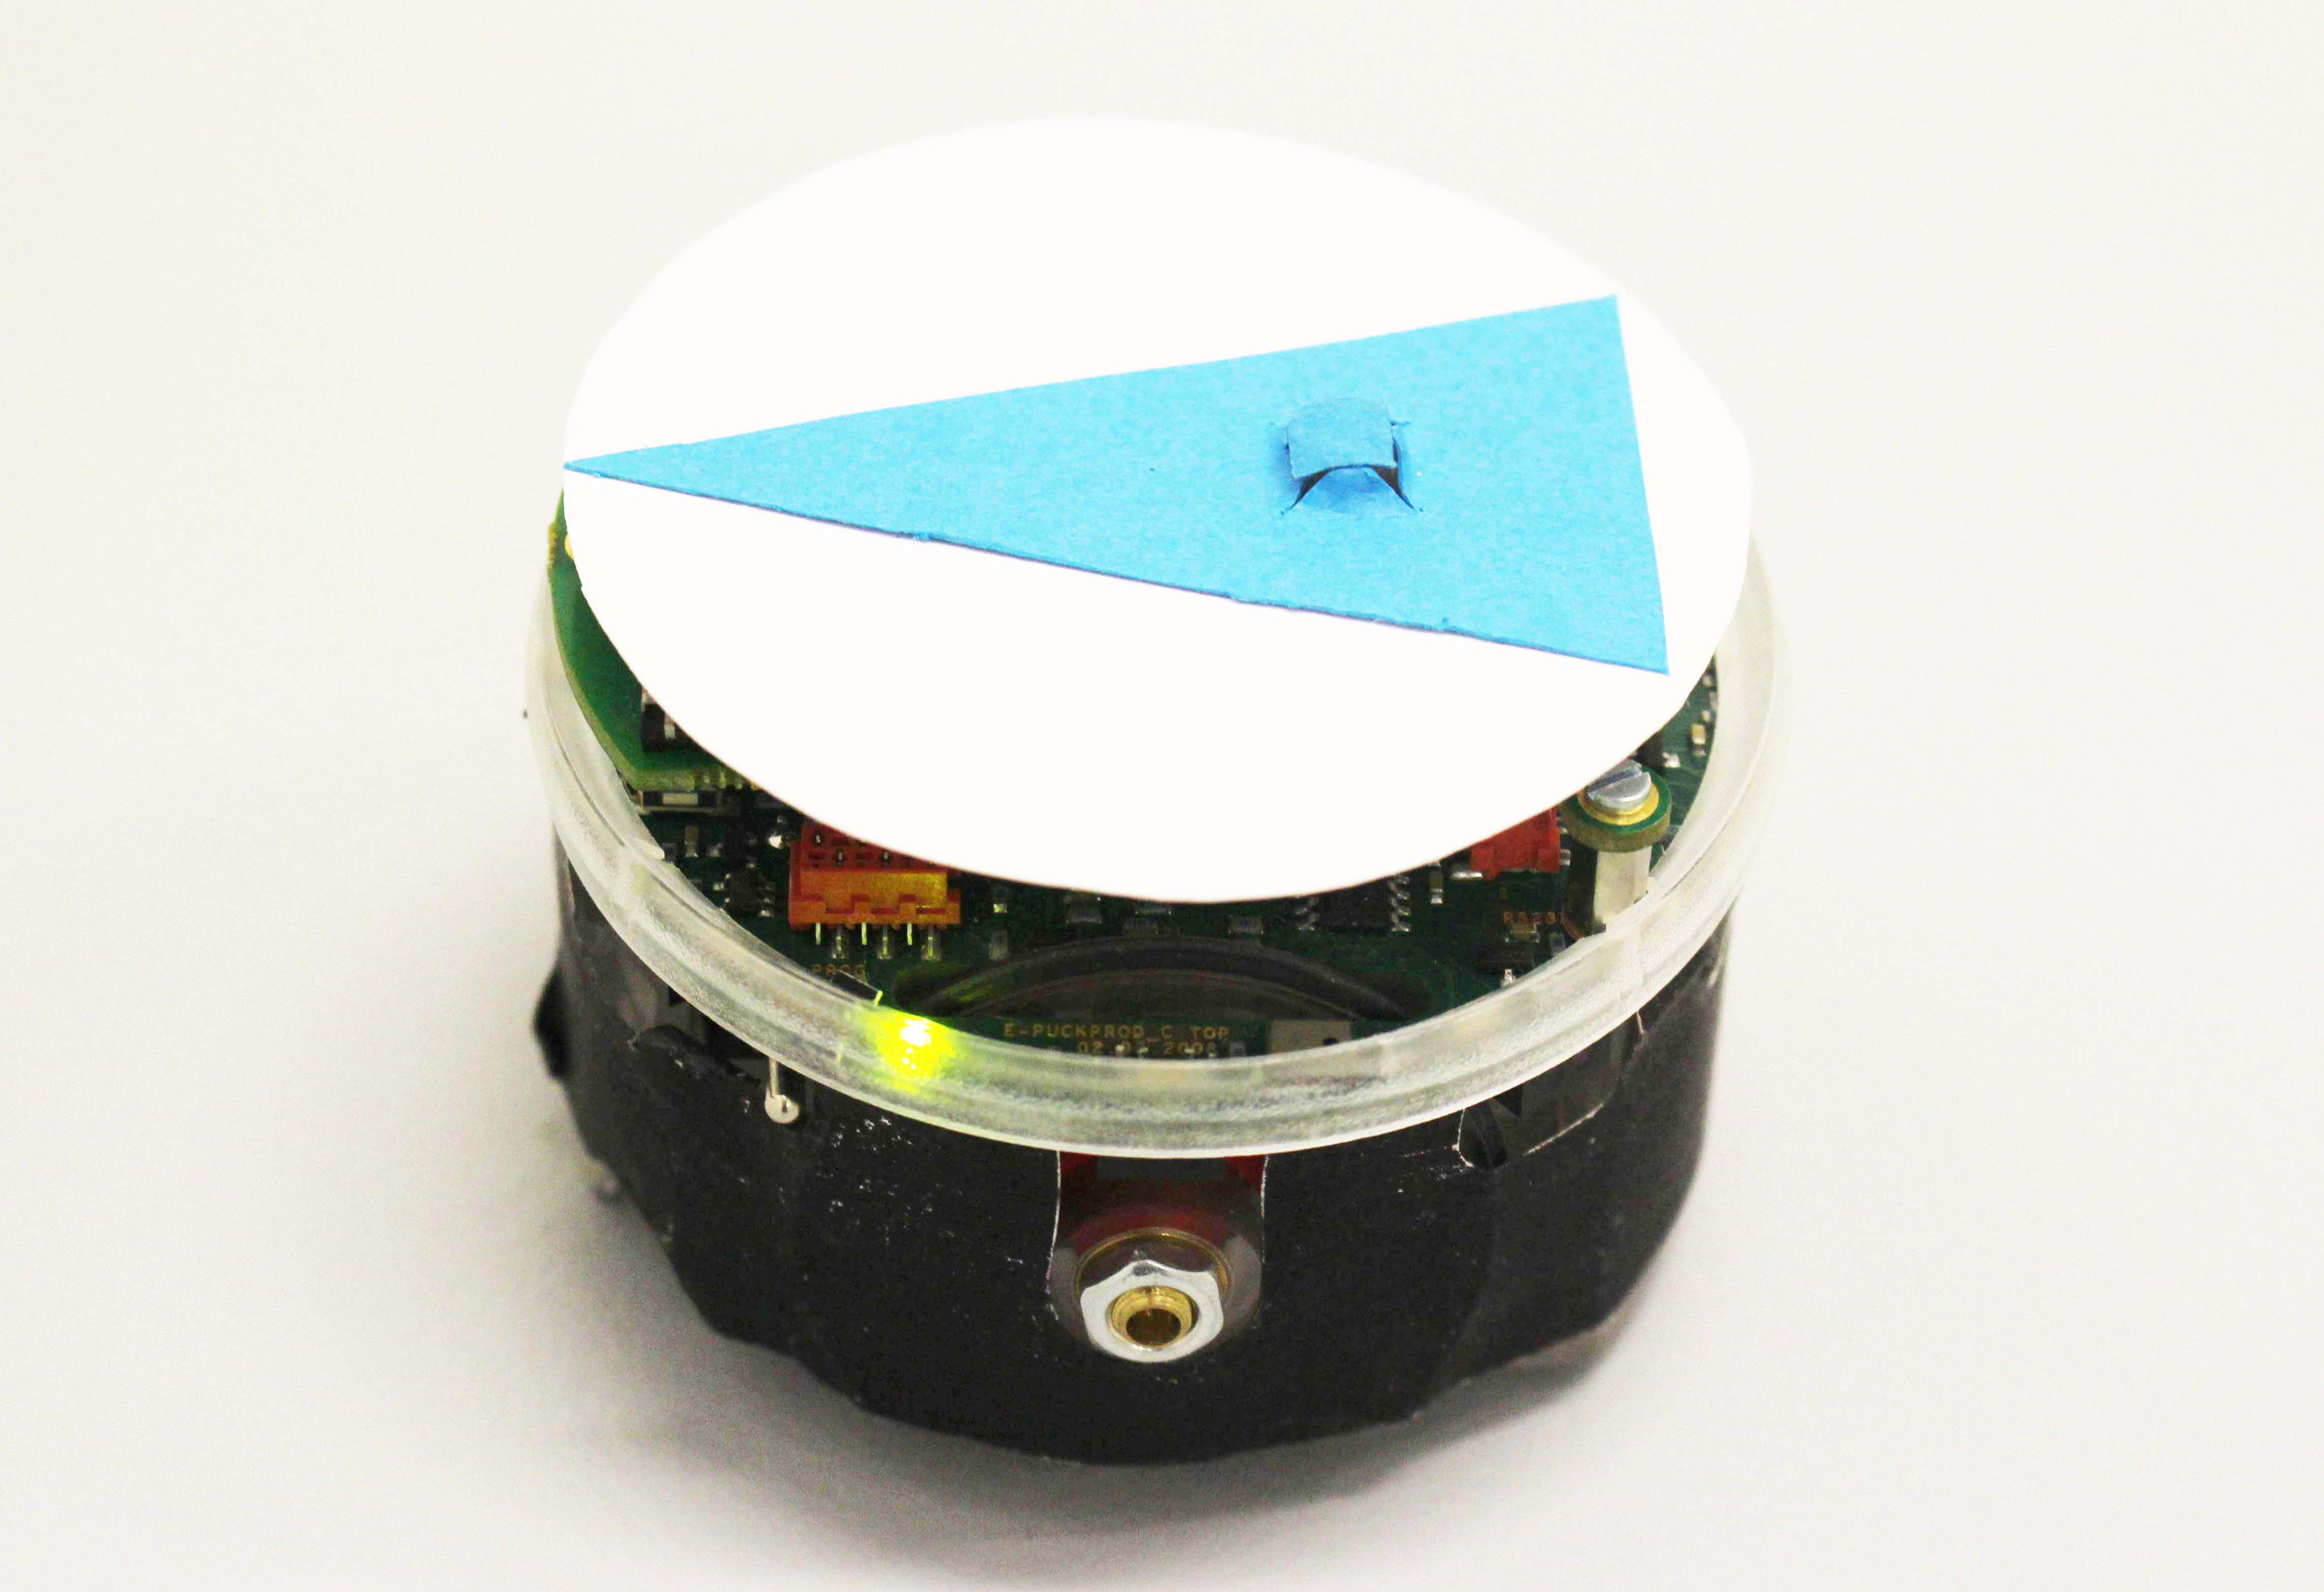
\includegraphics[width=3.5in]{e-puck_body.png}  %2.6
	\caption{An e-puck robot fitted with a black `skirt' and a top marker for motion tracking.}
	\label{fig:e-puck_body}
\end{figure}
%
\captionsetup[subfigure]{labelformat=empty}  
\begin{figure}[!t]
	\centering
	\subfloat[ \scriptsize{initial configuration}]{
		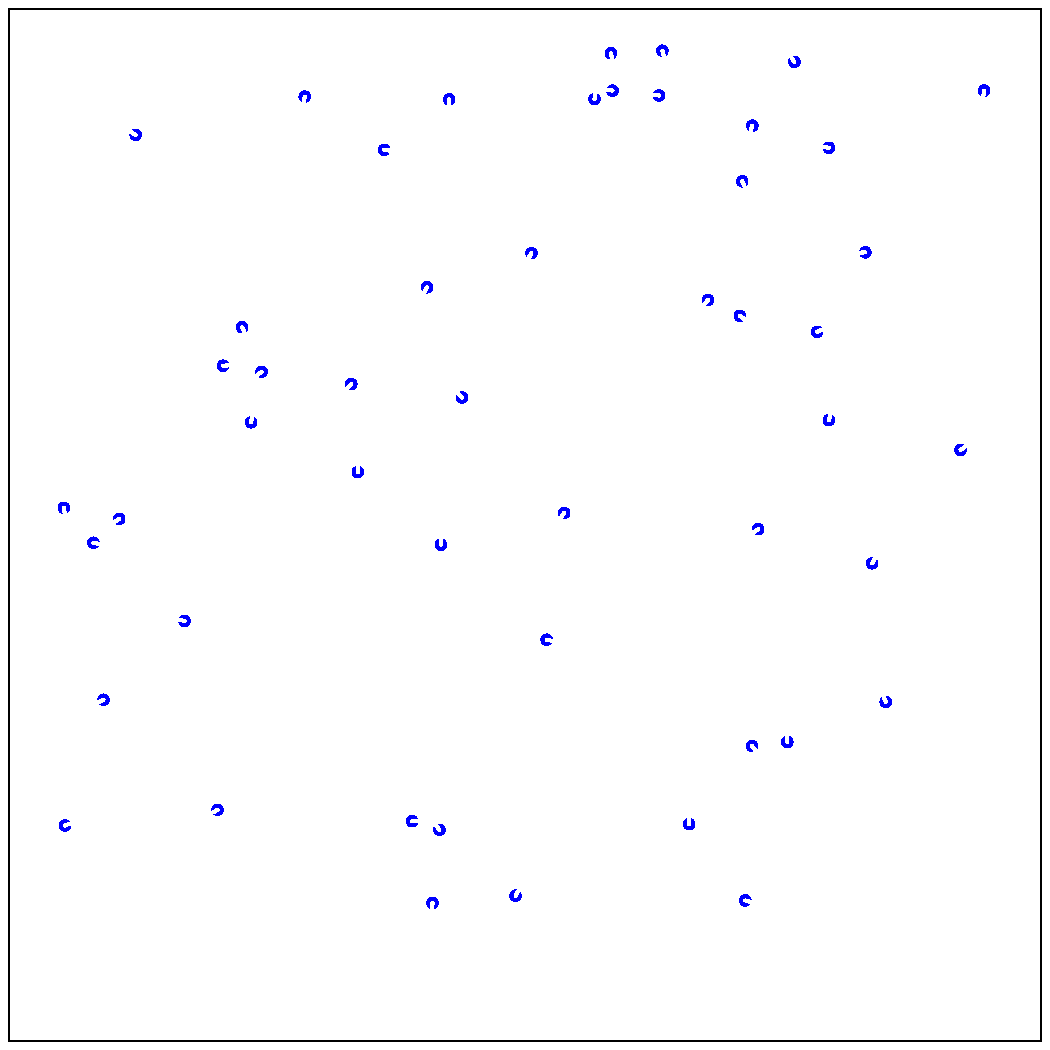
\includegraphics[width = 1.75 in]{snapshot_aggregation_initial.pdf}  %1.25
	}
	\subfloat[\scriptsize{after $60$ $\unit{s}$}]{
		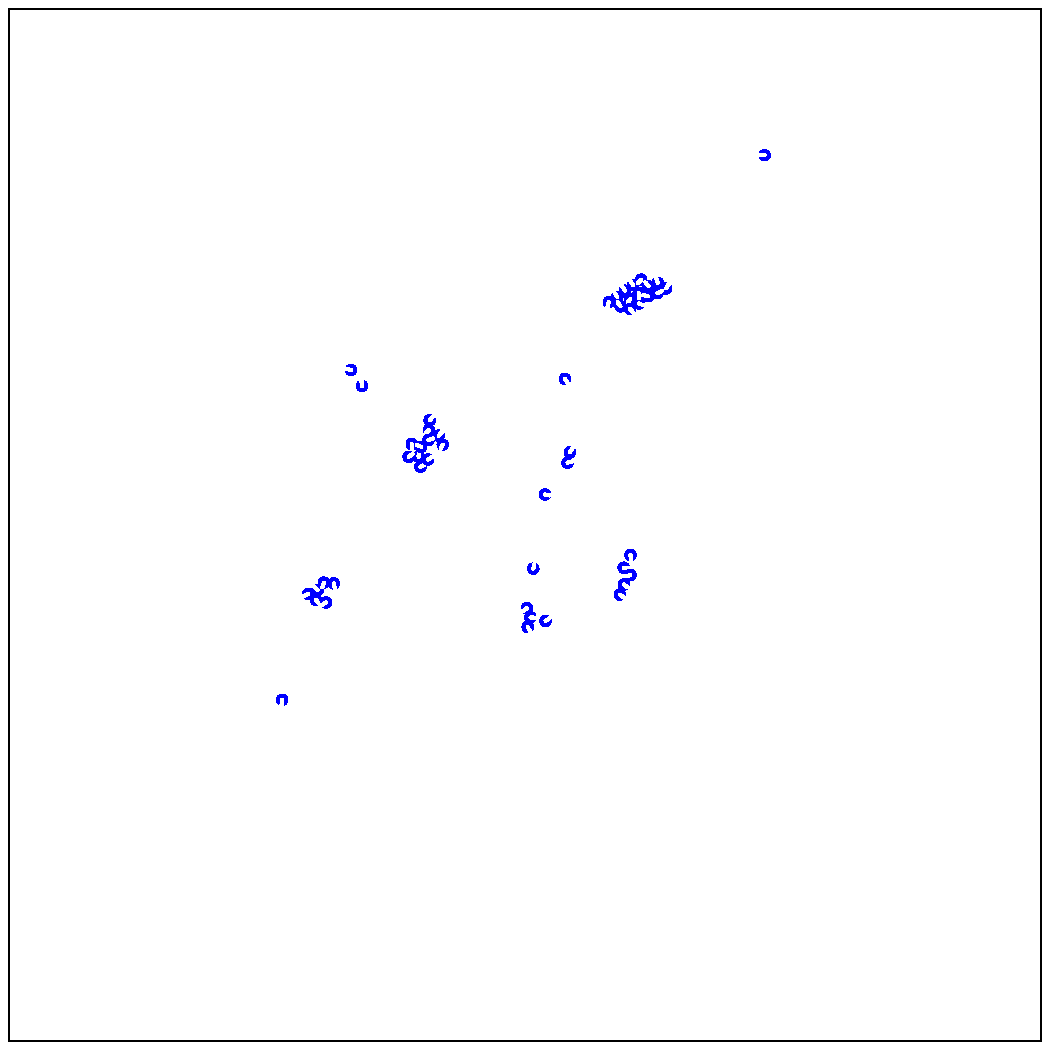
\includegraphics[width = 1.75 in]{snapshot_aggregation_60s.pdf}
	}\\
	\subfloat[\scriptsize{after $180$ $\unit{s}$}]{
		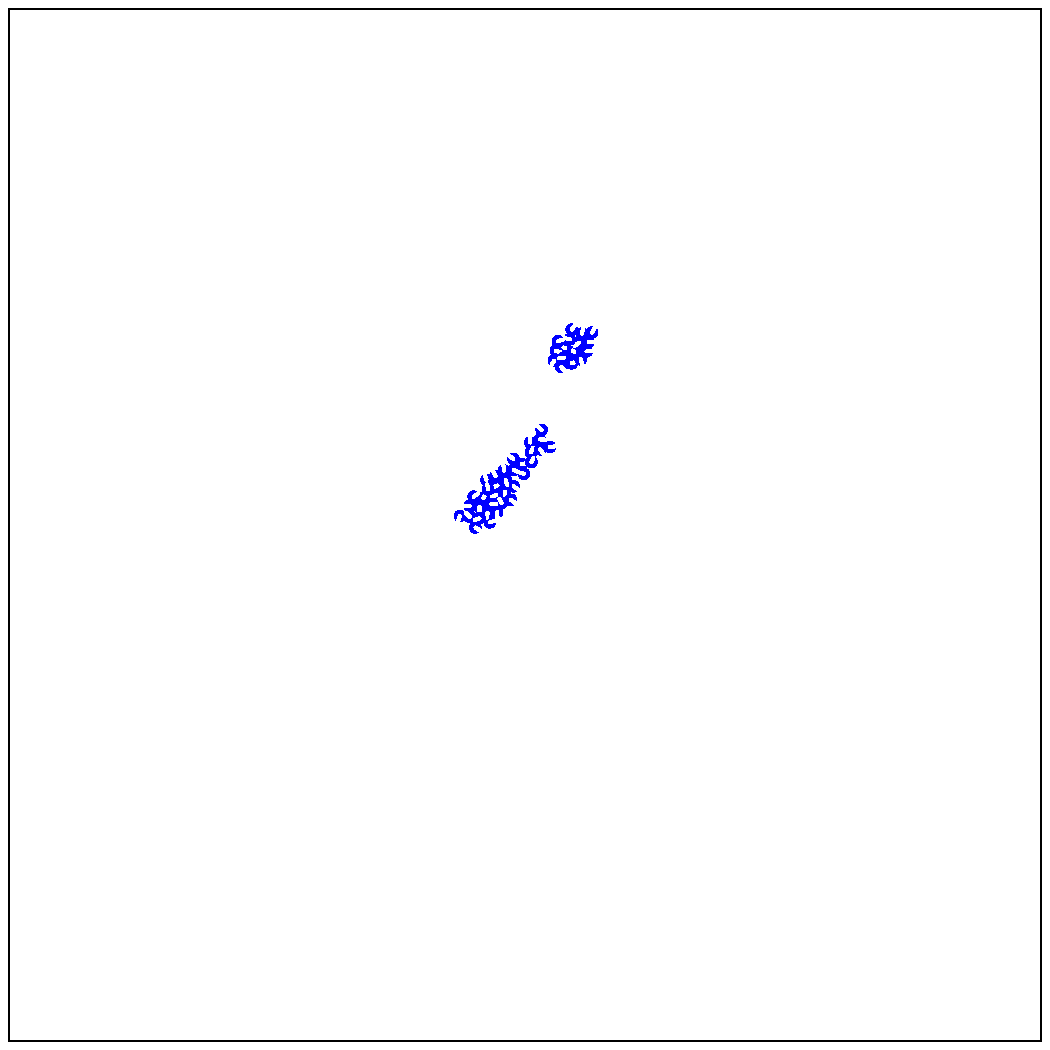
\includegraphics[width = 1.75 in]{snapshot_aggregation_180s.pdf}
	}
	\subfloat[\scriptsize{after $300$ $\unit{s}$}]{
		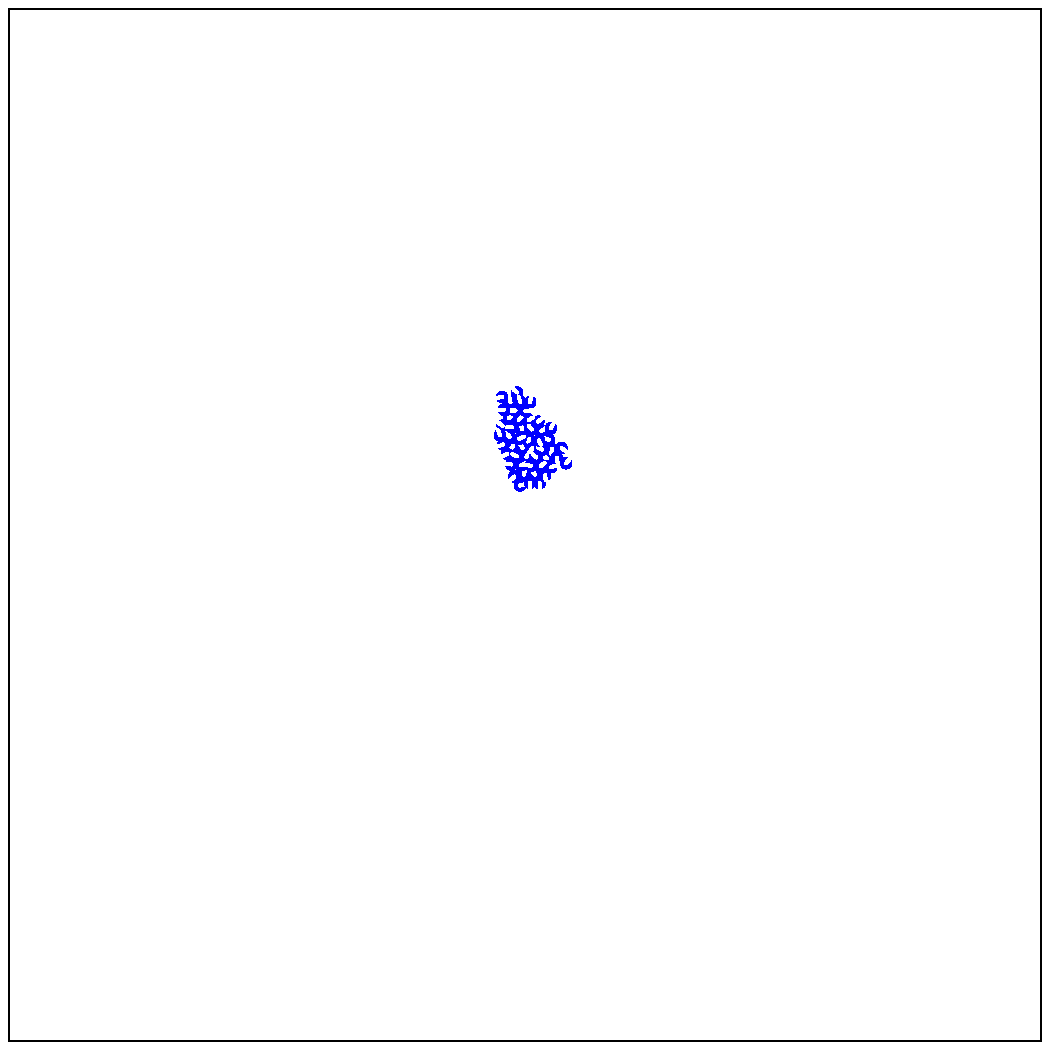
\includegraphics[width = 1.75 in]{snapshot_aggregation_300s.pdf}
	}
	\caption{Snapshots of the aggregation behavior of $50$ agents in simulation. }
	\label{fig:aggregation_snapshoot}
\end{figure}

The classifier does not have any prior knowledge about the individual under investigation. It is fed with the sequence of motion data of the individual. It has two input neurons ($i=2$), five hidden neurons ($h=5$) and one output neuron. The input neurons represent the linear speed ($v$) and angular speed ($\omega$) of the individual. They are obtained by tracking the positions and orientations of individuals. In simulation, the tracking is noise-free (situations with noise being
present are considered in Section~\ref{sec:noise_study_swarm_simulation} and the physical experiments in Chapter~\ref{ch:swarm_physical_implementation} where noise is inherently present). We define the linear speed to be positive when the angle between the individual's orientation and its direction of motion is smaller than $\unit[\pi \small/ 2]{rad}$, and negative otherwise. %This number was chosen arbitrarily and we did not attempt to optimize the number required. 

In the following, we detail the behavioral rules of the two swarm behaviors.

\captionsetup[subfigure]{labelformat=empty}  
\begin{figure}[!t]
	\centering
	\subfloat[\scriptsize{initial configuration}]
	{
		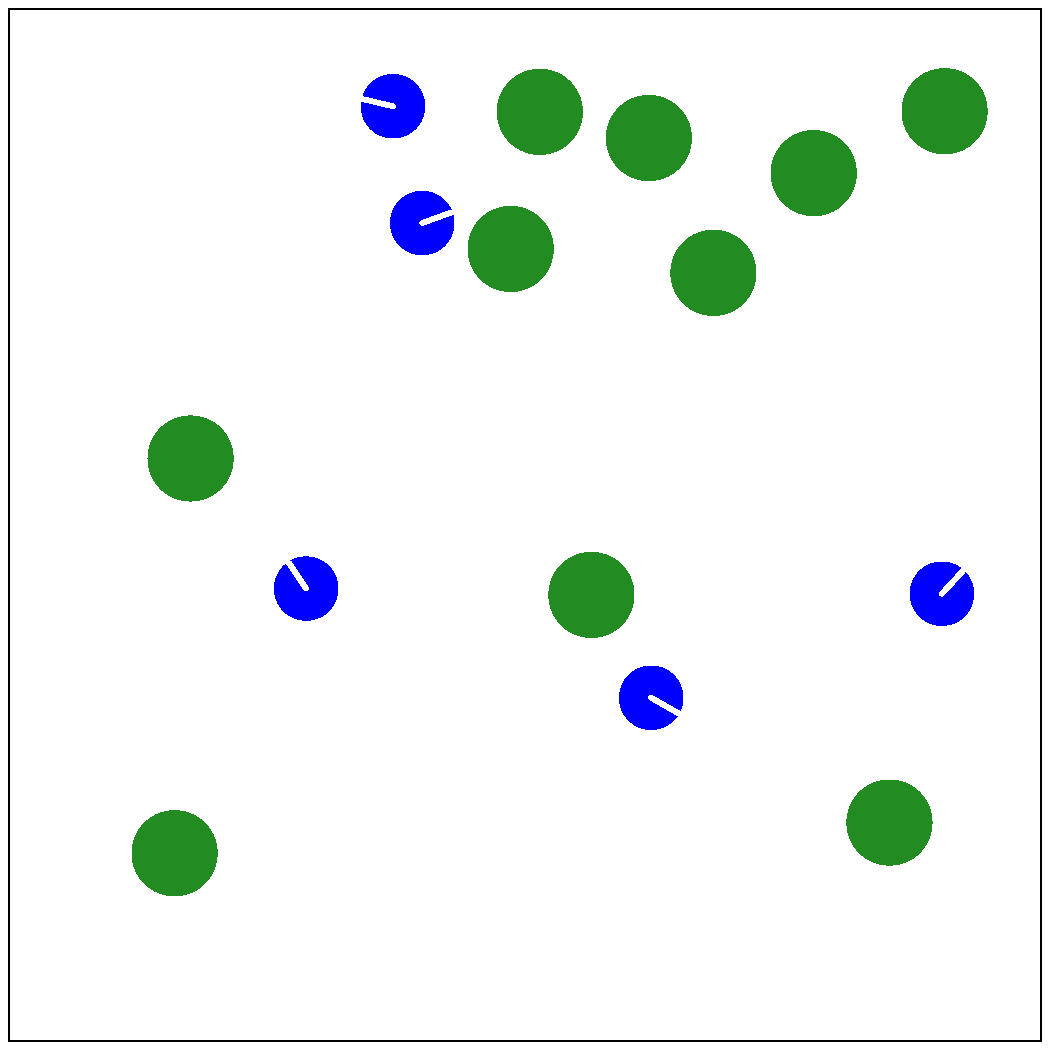
\includegraphics[width = 1.75 in]{snapshot_clustering_initial.pdf}  %1.25
	}
	\subfloat[\scriptsize{after $20$ $\unit{s}$}]{
		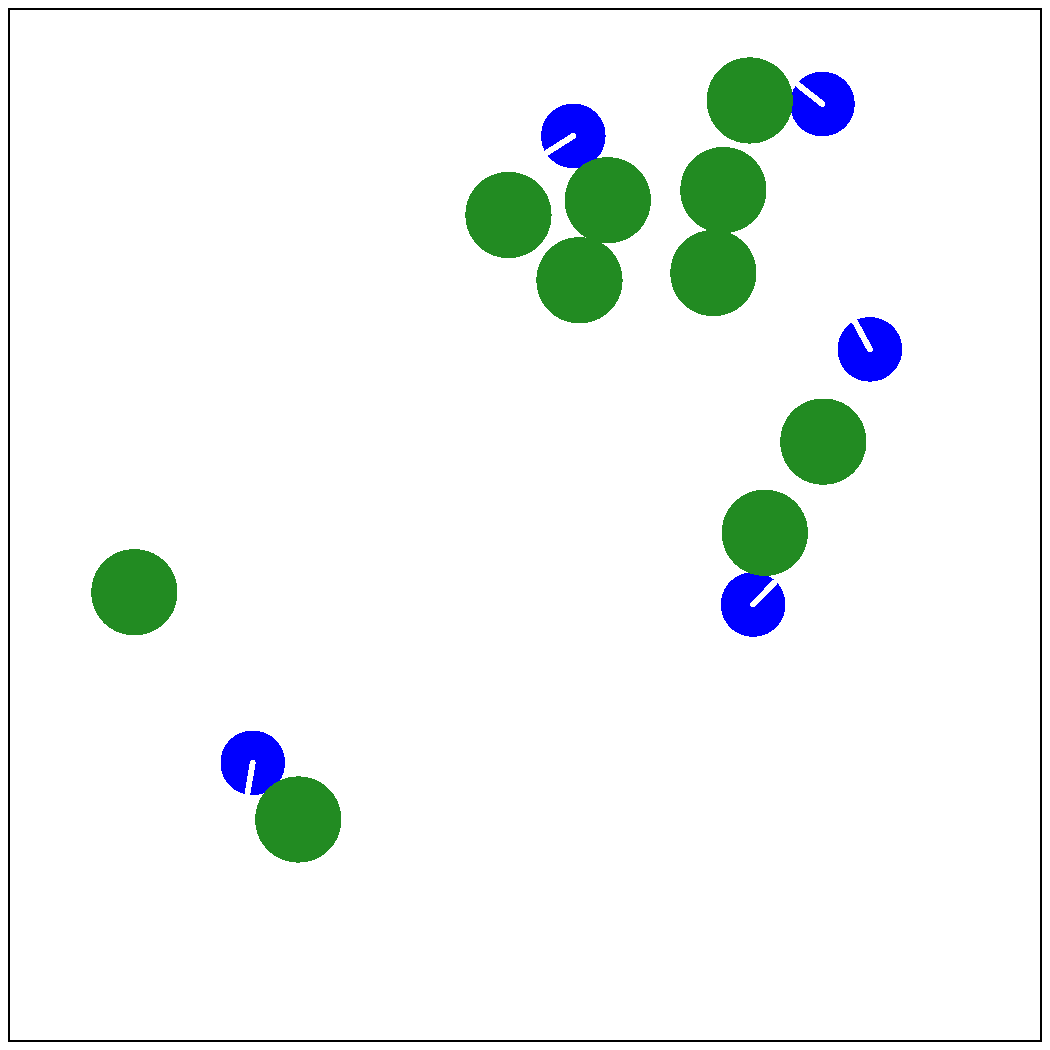
\includegraphics[width = 1.75 in]{snapshot_clustering_20s.pdf}
	}\\
	\subfloat[\scriptsize{after $40$ $\unit{s}$}]{
		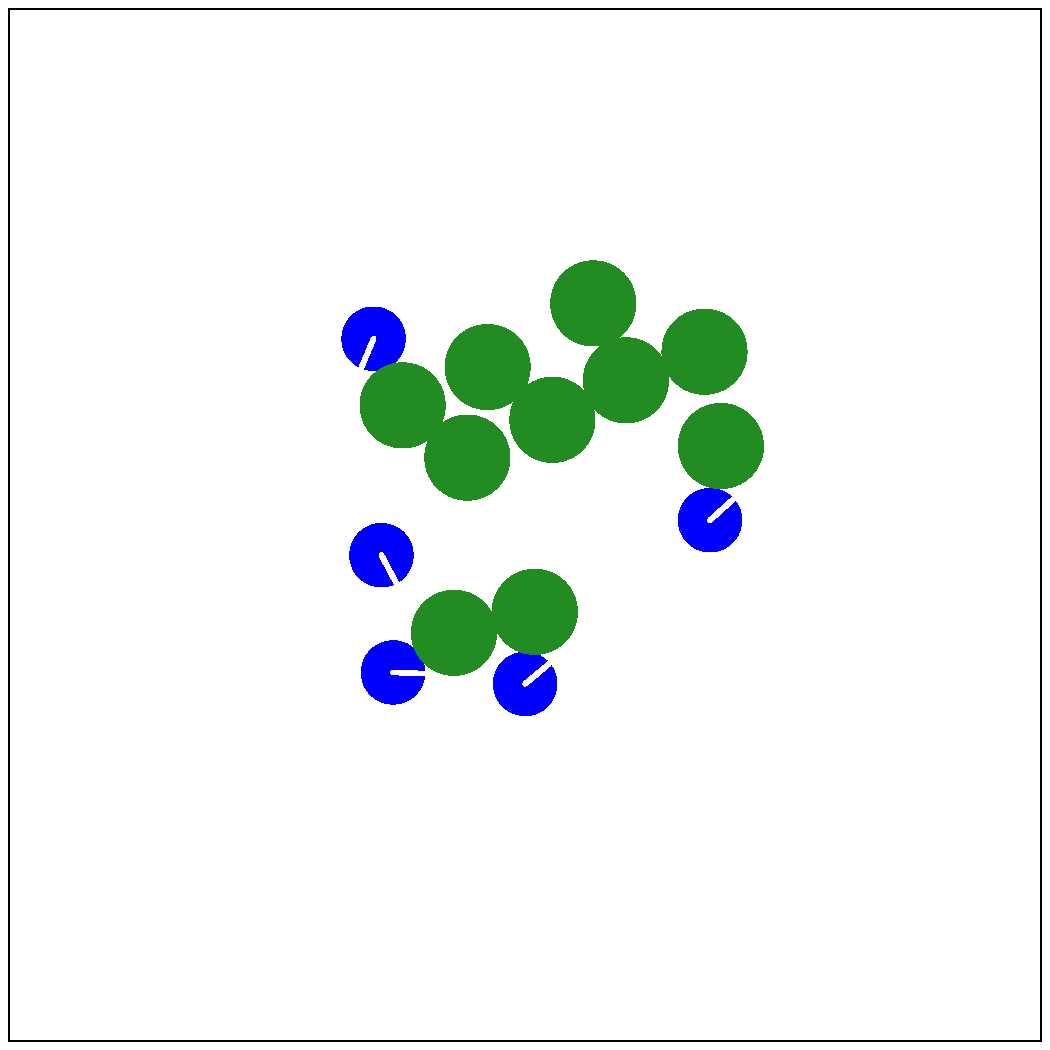
\includegraphics[width = 1.75 in]{snapshot_clustering_40s.pdf}
	}
	\subfloat[\scriptsize{after $60$ $\unit{s}$}]{
		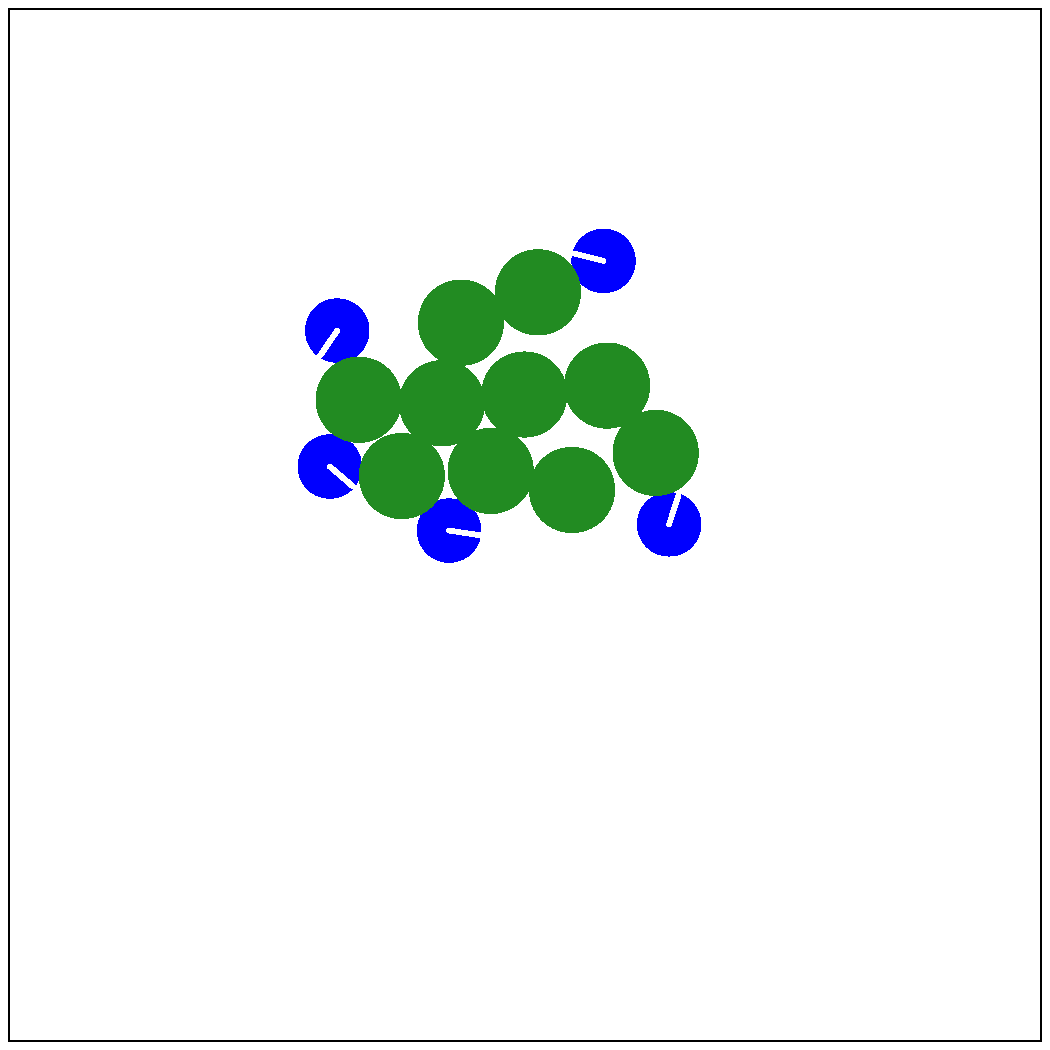
\includegraphics[width = 1.75 in]{snapshot_clustering_60s.pdf}
	}\\
	\caption{Snapshots of the object clustering behavior in simulation. There are $5$ agents (blue) and 10 objects (green).}
	\label{fig:clustering_snapshoot}
\end{figure}

\subsubsection{Aggregation}\label{sec:aggregation_behavior}
%
In this behavior, the sensor is binary, that is, $n=2$. It gives a reading of $I=1$ if there is an agent in the line of sight, and $I=0$ otherwise. The environment is free of obstacles. The objective for the agents is to aggregate into a single compact cluster as fast as possible. Further details, including a validation with 40 physical e-puck robots, are reported in~\cite{Gauci2014_ijrr}. %The agents are homogeneous: they all execute the same behavior. 

The `optimal' controller for aggregation was found by performing a grid search over the entire space of possible controllers (with finite resolution)~\cite{Gauci2014_ijrr}. The `optimal' controller's parameters are:
\begin{equation}\label{eq:aggregation_optimal_controller}
\mathbf{p} = \left(-0.7, -1.0, 1.0, -1.0\right). 
\end{equation}

When $I=0$, an agent moves backwards along a clockwise circular trajectory ($v_{\ell0} = -0.7$ and $v_{r0} = -1.0$). When $I=1$, an agent rotates clockwise on the spot with maximum angular velocity ($v_{\ell1} = 1.0$ and $v_{r1} = -1.0$). Note that rather counter-intuitively, an agent never moves forward, regardless of $I$. With this controller, an agent provably aggregates with another agent or a quasi-static cluster of agents~\cite{Gauci2014_ijrr}. Figure~\ref{fig:aggregation_snapshoot} shows snapshots from a simulation trial with $50$ agents.

\subsubsection{Object Clustering}
This behavior uses $n=3$ sensor states: $I=0$ if the sensor is pointing at the background (e.g., the wall of the environment, if the latter is bounded), $I=1$ if the sensor is pointing at an object, and $I=2$ if it is pointing at another agent. The objective of the agents is to arrange the objects into a single compact cluster as fast as possible. Details of this behavior, including a validation using 5 physical e-puck robots and 20 cylindrical objects, are presented in~\cite{Melvin2014_aamas}.

The controller's parameters, found using an evolutionary algorithm~\cite{Melvin2014_aamas}, are:
\begin{equation}\label{eq:clustering_optimal_controller}
\mathbf{p} = \left( 0.5, 1.0, 1.0, 0.5, 0.1, 0.5 \right).
\end{equation} 

When $I=0$ and $I=2$, the agent moves forward along an anti-clockwise circular trajectory, but with different linear and angular speeds. When $I=1$, it moves forward along a clockwise circular trajectory. Figure~\ref{fig:clustering_snapshoot} shows snapshots from a simulation trial with $5$ agents and $10$ objects.

\section{Simulation Platform and Setups}\label{sec:simulation_platform_setups}
 
In this section, we present the agent platform for simulating the two swarm behaviors under investigation and the simulation setups for performing coevolution runs.

\subsection{Simulation Platform}\label{sec:platform_swarm_simulation}

We use the open-source Enki library~\cite{Enki}, which models the kinematics and dynamics of rigid objects, and handles collisions. Enki has a built-in 2-D model of the e-puck. The robot is represented as a disk of diameter $\unit[7.0]{cm}$ and mass $\unit[150]{g}$. The inter-wheel distance is $\unit[5.1]{cm}$. The speed of each wheel can be set independently. Enki induces noise on each wheel speed by multiplying the set value by a number in the range $(0.95, 1.05)$ chosen randomly with uniform distribution. The maximum speed of the e-puck is $\unit[12.8]{\textrm{cm/s}}$, forward or backward. The line-of-sight sensor is simulated by casting a ray from the e-puck's front and checking the first item with which it intersects (if any). The range of this sensor is unlimited in simulation. 
%Although Enki models the e-puck's real sensors, we choose to implement the line-of-sight sensor independently, for the sake of accuracy (in the physical experiments, this sensor is realized using the e-puck's camera; see Section~\ref{sec:robot_platform_sensor_implementation}).

In the object clustering case study, we model objects as disks of diameter $\unit[10]{cm}$ with mass $\unit[35]{g}$ and a coefficient of static friction with the ground of $0.58$, which makes it movable by a single e-puck.

The robot's control cycle is updated every $\unit[0.1]{s}$, and the physics is updated every $\unit[0.01]{s}$.

\subsection{Simulation Setups}\label{sec:setup_swarm_simulation}

In all simulations, we used an unbounded environment. For the aggregation case study, we used groups of $11$ individuals---$10$ agents and $1$ replica that executes a model. The initial positions of individuals were generated randomly in a square region of sides $\unit[331.66]{cm}$, following a uniform distribution (average area per individual = $\unit[10000]{cm^2}$). For the object clustering case study, we used groups of $5$ individuals---$4$ agents and $1$ replica that executes a model---and $10$ cylindrical objects. The initial positions of individuals and objects were generated randomly in a square region of sides $\unit[100]{cm}$, following a uniform distribution (average area per object = $\unit[1000]{cm^2}$). In both case studies, individual starting orientations were chosen randomly in $[-\pi,\pi]$ with uniform distribution. %The initial configuration\footnote{Throughout this chapter, `initial configuration' refers to initial positions and orientations of the individuals or objects, if any.} of the individuals is randomly generated in each trial. 

We performed 30 coevolution runs for each case study. Each run lasted 1000 generations. The model and classifier populations each consisted of $100$ solutions ($\mu = 50$,  $\lambda = 50$). In each trial, classifiers observed individuals for $\unit[10]{s}$ at $\unit[0.1]{s}$ intervals ($100$ data points). 

\begin{figure}[!t]%htbp
	\centering
		\subfloat[(a) Aggregation \label{fig:model_parameters_box_aggregation}]{%
			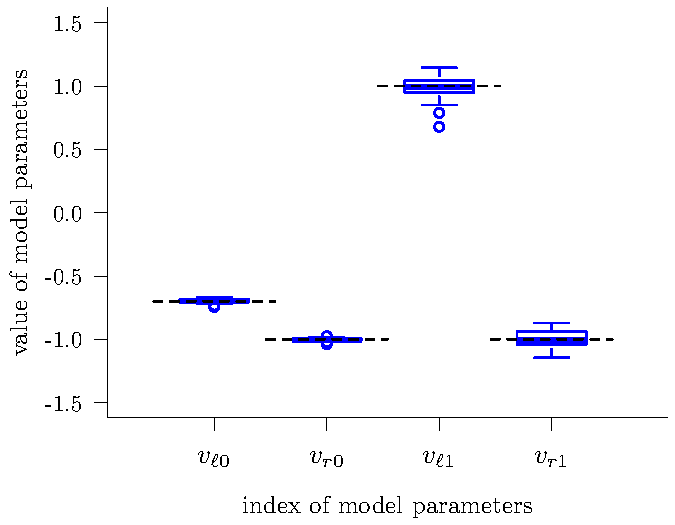
\includegraphics[width=3.5 in]{model_parameters_box_aggregation.pdf}
		}\\
		\subfloat[(b) Object Clustering\label{fig:model_parameters_box_clustering}]{%
			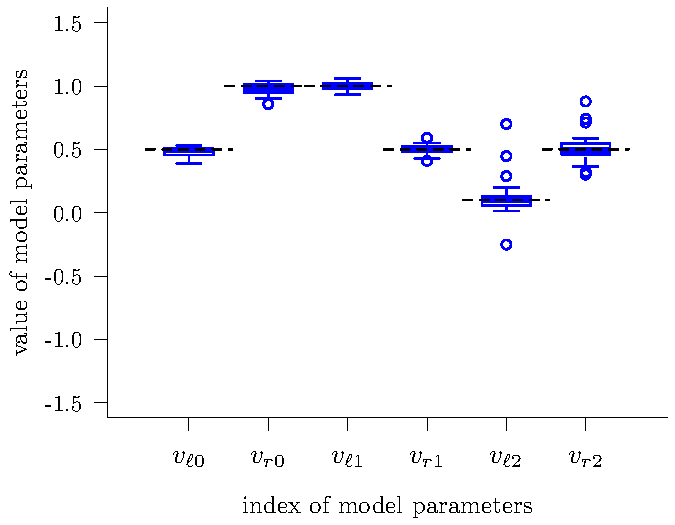
\includegraphics[width=3.5 in]{model_parameters_box_clustering.pdf}
		}
		\caption{Parameters of the evolved models with the highest subjective fitness in the $1000^\textrm{th}$ generation in the coevolutions for (a) the aggregation behavior and (b) the object clustering behavior. Each box corresponds to 30 coevolution runs in simulation. The dotted black lines correspond to the values of the parameters that the system is expected to learn (i.e., those of the agent).\label{fig:model_parameters_box}}
\end{figure}
%

\section{Simulation Results}\label{sec:results_swarm_simulation}

\subsection{Analysis of Evolved Models}\label{sec:analysis_evolved_models_swarm_simulation}

In order to objectively measure the quality of the models obtained through~\textit{Turing Learning}, we define two metrics. Given an evolved controller (model) $\mathbf{x}$ and the original agent controller $\mathbf{p}$, where $\mathbf{x},\mathbf{p}\in[-1,1]^{2n}$, we define the absolute error (AE) in a particular parameter $i\in\{1,2,\dots,2n\}$ as: 
\begin{equation}\label{eq:AE}
\mathrm{AE}_i = |x_i-p_i|. 
\end{equation}

We define the mean absolute error (MAE) over all parameters as: 
\begin{equation}\label{eq:MAE}
\mathrm{MAE} = \frac{1}{2n}\sum_{i=1}^{2n} \mathrm{AE}_i.
\end{equation}
%\footnote{Throughout the main text, we exclusively use the acronyms AE and MAE. Therefore ``mean AE'' is not to be confused with MAE; rather, it refers to the mean AE in one parameter over a number of coevolution runs.}

Fig.~\ref{fig:model_parameters_box} shows a box plot\footnote{The box plots presented here are all as follows. The line inside the box represents the median of the data. The edges of the box represent the lower and the upper quartiles of the data, whereas the whiskers represent the lowest and the highest data points that are within $1.5$ times the range from the lower and the upper quartiles, respectively. Circles represent outliers.\label{fn:boxplot}} with the parameters of the evolved models with the highest subjective fitness\footnote{The fitness of the models depends solely on the judgments of the classifiers from the competing population, and is hence referred to as \textit{subjective}.} in the final generation. It can be seen that~\textit{Turing Learning} identified the parameters for both behaviors with good accuracy (dotted black lines represent the ground truth, that is, the parameters of the observed swarming agents). In the case of aggregation, the means (standard deviations) of the AEs in the parameters were (from left to right in Fig.~\subref*{fig:model_parameters_box_aggregation}): $0.01$ ($0.01$), $0.01$ ($0.01$), $0.07$ ($0.07$) and $0.06$ ($0.04$). In the case of object clustering, these values were: $0.03$ ($0.03$), $0.04$ ($0.03$), $0.02$ ($0.02$), $0.03$ ($0.03$), $0.08$ ($0.13$) and $0.08$ ($0.09$).
%In the rest of this thesis, unless otherwise stated, `evolved model' refers to the model with the highest subjective fitness in a generation.

We also investigated the evolutionary dynamics. Fig.~\ref{fig:model_parameters_convergence} shows how the model parameters converged over generations. In the aggregation case study, the parameters corresponding to $I=0$ were learned first. After around $50$ generations, both $v_{\ell0}$ and $v_{r0}$ closely approximated their true values ($-0.7$ and $-1.0$), shown in Fig.~\subref*{fig:model_parameters_convergence_aggregation}. For $I=1$, it took about $200$ generations for both $v_{\ell1}$ and $v_{r1}$ to converge. A likely reason for this effect is that an agent spends a larger proportion of its time seeing nothing ($I=0$) than other agents ($I=1$)---simulations revealed these percentages to be $91.2\%$ and $8.8\%$, respectively (mean values across $100$ trials). 

In the object clustering case study, the parameters corresponding to $I=0$ and $I=1$ were learned faster than the parameters corresponding to $I=2$, as shown in Fig.~\subref*{fig:model_parameters_convergence_clustering}. After about $200$ generations, $v_{\ell0}$, $v_{r0}$, $v_{\ell1}$ and $v_{r1}$ started to converge; however it took about $400$ generations for $v_{\ell2}$ and $v_{r2}$ to approximate their true values. Note that an agent spends the highest proportion of its time seeing nothing ($I=0$), followed by objects ($I=1$) and other agents ($I=2$)---simulations revealed these proportions to be $53.2\%$, $34.2\%$ and $12.6\%$, respectively (mean values across $100$ trials).
\begin{figure}[!t]%
	\centering
		\subfloat[(a) Aggregation \label{fig:model_parameters_convergence_aggregation}]{%
			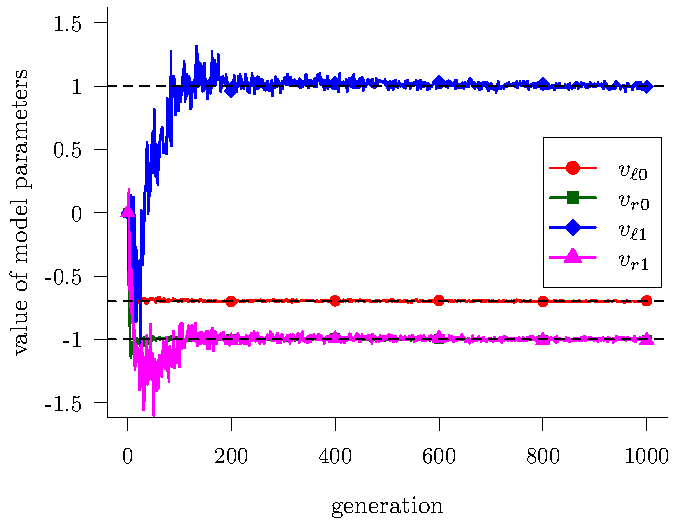
\includegraphics[width=3.5 in]{model_parameters_convergence_aggregation.pdf}
		}\\
		\subfloat[(b) Object Clustering\label{fig:model_parameters_convergence_clustering}]{%
			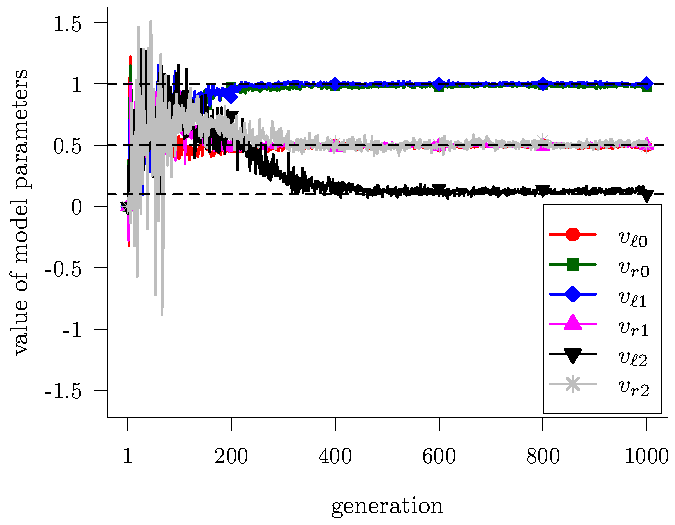
\includegraphics[width=3.5 in]{model_parameters_convergence_clustering.pdf}
		}
		\caption{Evolutionary process of the evolved model parameters for (a) the aggregation behavior and (b) the object clustering behavior. Curves represent median values across 30 coevolution runs. Dotted black lines indicate true values. \label{fig:model_parameters_convergence}}
\end{figure}

\begin{figure}[!t]
	\centering
		\subfloat[(a) Aggregation \label{fig:model_validation_aggregation_simulation}]{%
			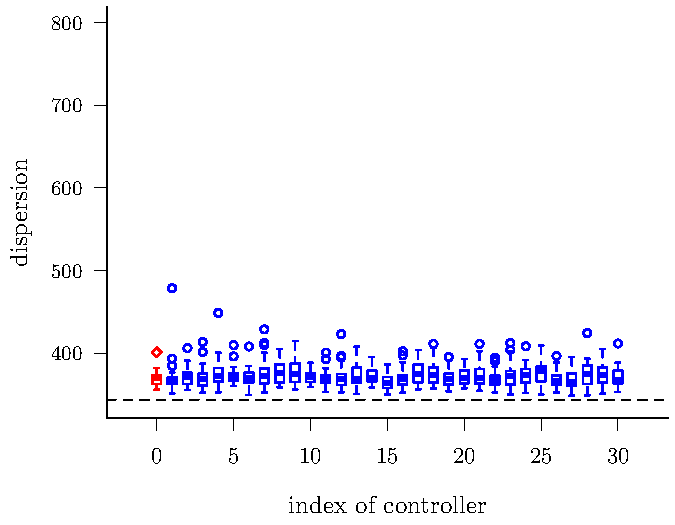
\includegraphics[width=3.5 in]{model_validation_aggregation_simulation.pdf}
		}\\
		\subfloat[(b) Object Clustering\label{fig:model_validation_clustering_simulation}]{%
			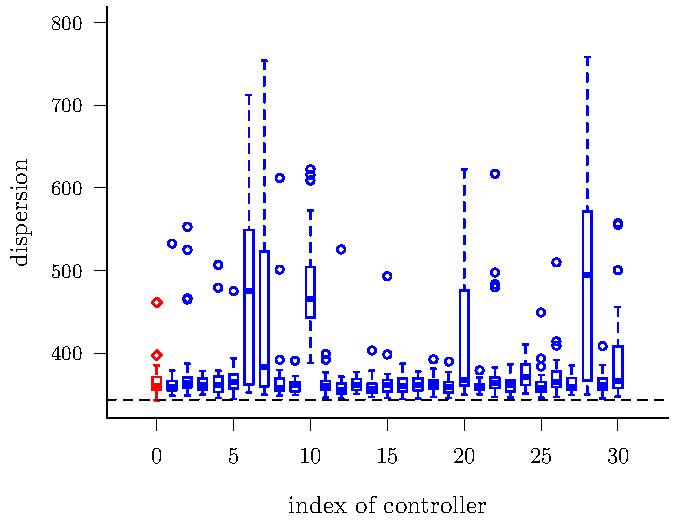
\includegraphics[width=3.5 in]{model_validation_clustering_simulation.pdf}
		}
		\caption{(a) Dispersion (after $\unit[400]{s}$) of $50$ agents executing the original aggregation controller (red box) or one of the $30$ evolved models (blue boxes) of the $1000^\mathrm{th}$ generation. (b) Dispersion (after $\unit[400]{s}$) of $50$ objects in a swarm of $25$ agents executing the original object clustering controller (red box) or one of the $30$ evolved models (blue boxes). In both (a) and (b), boxes show distributions over $30$ trials. The dotted black lines indicate the minimum dispersion that $50$ agents/objects can possible achieve~\cite{Graham1990}. See Section~\ref{sec:analysis_evolved_models_swarm_simulation} for details.\label{fig:model_validation_simulation}}
\end{figure}

Although the evolved models approximate the agents well in terms of parameters, it has often been observed in swarm systems that small changes in individual agent behaviors can lead to vastly different emergent behaviors, especially with large numbers of agents~\cite{Paul2010}. For this reason, we evaluated the quality of the emergent behaviors that the models give rise to. In the case of aggregation, a good measure of the emergent behavior is the dispersion of the swarm after some elapsed time as defined in~\cite{Gauci2014_ijrr}\footnote{The measure of dispersion is based on the robots'/objects' distances from their centroid. For a formal definition, see Equation (5) of \cite{Gauci2014_ijrr}, Equation (2) of~\cite{Melvin2014_aamas} and~\cite{Graham1990}.}. For each of the $30$ models with the highest subjective fitness in the final generation, we performed $30$ trials with $50$ agents each executing the model. For comparison, we also performed $30$ trials using the original controller (see Equation~\eqref{eq:aggregation_optimal_controller}). The set of initial configurations was the same for all models and the original controller. Fig~\subref*{fig:model_validation_aggregation_simulation} shows the dispersion for the original controller and models after $\unit[400]{s}$. All models led to aggregation. We performed a statistical test\footnote{Throughout this thesis, the statistical test used is a two-sided Mann-Whitney test with a $5\%$ significance level.} on the final dispersion of the agents between the original controller and each model. There was no statistically significant difference in $26$ out of $30$ cases ($30$ out of $30$ cases with Bonferroni correction). 
%in individual agent behaviors can lead to vastly different emergent behaviors, especially with large numbers of agents~\cite{Paul2010, Luca2014}

In the case of object clustering, we use the dispersion of the objects after some elapsed time as a measure of the emergent behavior. With the original controller (see Equation~\eqref{eq:clustering_optimal_controller}) and each of the models, we performed $30$ trials with $25$ agents and $50$ objects. The results are shown in Fig.~\subref*{fig:model_validation_clustering_simulation}. In a statistical test on the final dispersion of the objects between the original controller and each model, there was no statistically significant difference in $24$ out of $30$ cases ($26$ out of $30$ cases with Bonferroni correction).

We also investigated the evolutionary process of the model parameters. Figure~\ref{fig:model_parameters_convergence} shows the convergence of the model parameters over generations. In the aggregation behavior, the parameters corresponding to $I=0$ were learned first. After about $50$ generations, both $v_{\ell0}$ and $v_{r0}$ closely approximated their true values ($-0.7$ and $-1.0$) shown in Figure~\subref*{fig:model_parameters_box_aggregation}. For $I=1$, it took about $200$ generations for both $v_{l1}$ and $v_{r1}$ to converge. A likely reason for this effect is that an agent spends a larger percentage of its time seeing nothing ($I=0$) than other agents ($I=1$)---simulations revealed these percentages to be $8.8\%$ and $91.2\%$, respectively (mean values over 100 trials). 

In the object clustering behavior, the parameters corresponding to $I=0$ and $I=1$ were learned faster than the other two parameters corresponding to $I=2$, as shown in the Figure~\subref*{fig:model_parameters_convergence_clustering}. After about $200$ generations, $v_{\ell0}$, $v_{r0}$, $v_{l1}$ and $v_{r1}$ started to converge; however it took about $400$ generations for $v_{l2}$ and $v_{r2}$ to approximate their true values. This is likely because an agent spends the most percentage of its time seeing nothing ($I=0$), followed by objects ($I=1$) and other agents ($I=2$)---simulations revealed these percentages to be $53.2\%$, $34.2\%$ and $12.6\%$ , respectively (mean values over 100 trials).

\begin{figure}[!t]%
	\centering
		\subfloat[(a) Aggregation \label{fig:fitness_curve_aggregation_simulation}]{%
			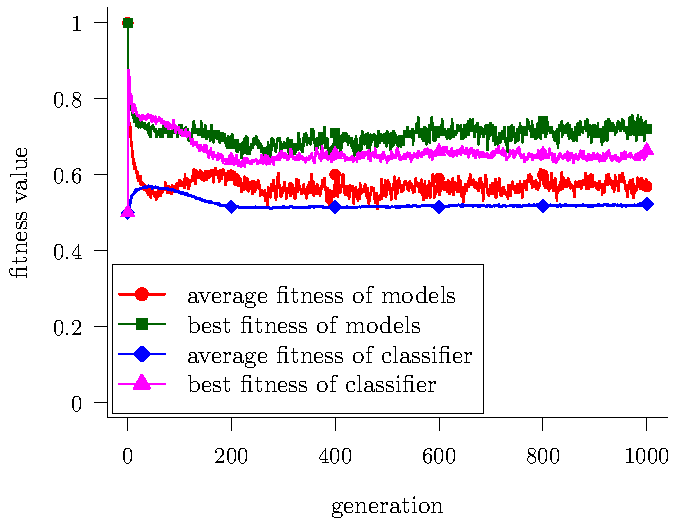
\includegraphics[width=3.5 in]{fitness_curve_aggregation_simulation.pdf}
		}\\
		\subfloat[(b) Object Clustering \label{fig:fitness_curve_clustering_simulation}]{%
			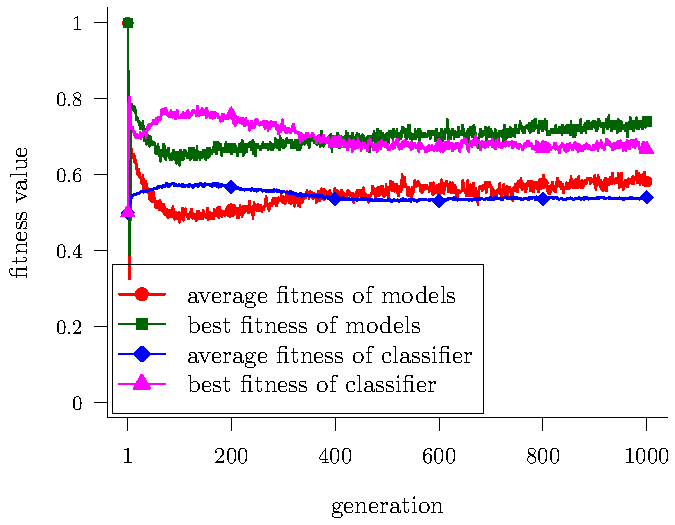
\includegraphics[width=3.5 in]{fitness_curve_clustering_simulation.pdf}
		}
		\caption{This plot shows the subjective fitness of the classifiers and
		the models for (a) the aggregation behavior and (b) the object clustering behavior.
		The curves show the median value across 30 coevolution runs.\label{fig:fitness_dynamics_simulation}}
\end{figure}

\subsection{Coevolutionary Dynamics}\label{sec:coevolutionary_dynamics_simulation_swarm_simulation}
In order to analyze how the classifiers and the models interact with each other during the course of the coevolution, we investigate the dynamics of the subjective fitness of the classifiers and the models as shown in Figure~\ref{fig:fitness_dynamics_simulation}. 

In the aggregation behavior, at the beginning, the fitness of the classifiers is 0.5 as they output 1 for all the agents and models, which means the classifiers make uninformed decisions\footnote{Note that in the implementation of the coevolutionary algorithm, the parameters of the models and classifiers are initialized to $0.0$, which means all the classifiers are identical at the $1^{\mathrm{st}}$ generation.}. Therefore, the fitness of the models starts from 1.0, as all the classifiers judge them the agent. Then, the average fitness of the classifiers quickly increases, corresponding to the decline of the average fitness of the models. As the models learn to adapt, the average fitness of the classifiers only increases slightly until about the $50^{\mathrm{th}}$ generation. After that, the average fitness of the models starts to increase. However, the best fitness of the classifiers is still higher than that of the models. The best fitness of the models surpasses that of the classifiers after about the $120^{\mathrm{th}}$ generation; at this point, the fitness of the `best' model (selected by the classifiers) is around $0.7$. This means that the `best' model is able to mislead $70\%$ of the classifiers into judging it as the agent. From the $200^{\mathrm{th}}$ generation onwards, the fitness of the classifiers and models remains ``balanced'' until the last generation. 

The coevolutionary dynamics of the object clustering behavior is similar. Compared with the dynamics of the aggregation behavior, it takes more generations for the fitness of the models to surpass that of the classifiers. This could be explained by the higher number of parameters and the higher complexity of the behavior to be evolved in the object clustering behavior.

\begin{figure}[!t]
	\centering
	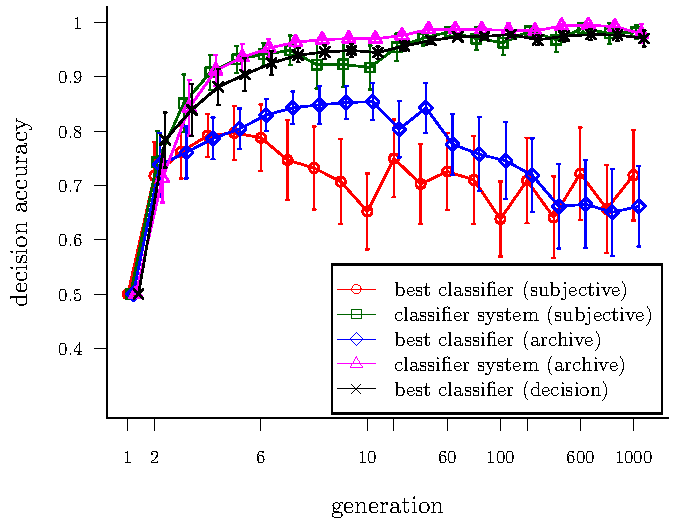
\includegraphics[width=3.5 in]{classifier_decision_accuracy_simulation.pdf}
	\caption{The average decision accuracy of the best classifiers and classifier systems over generations (nonlinear scale) in $30$ coevolution runs. The error bars show standard deviations. See text for details.}
	\label{fig:classifier_decision_accuracy_swarm_simulation}
\end{figure}

\begin{figure}[!t]
	\centering
	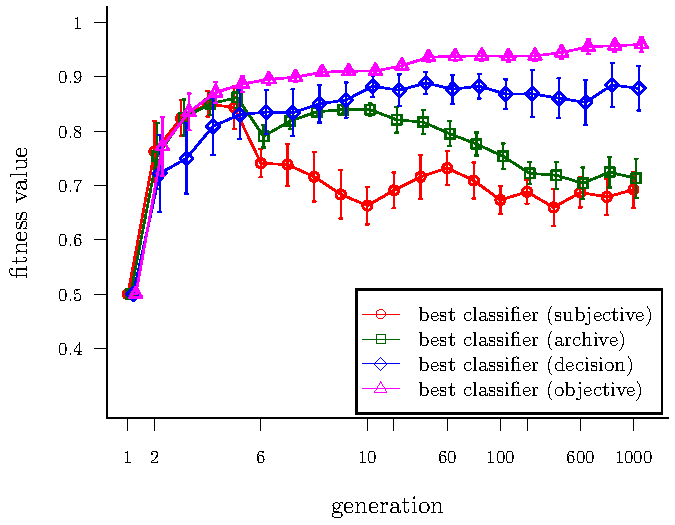
\includegraphics[width=3.5 in]{classifier_fitness_simulation.pdf}
	\caption{This plot shows the average fitness of the classifiers over generations (nonlinear scale) in $30$ coevolution runs. The fitness is calculated based on $14641$ testing models. See text for details.}
	\label{fig:classifier_fitness_swarm_simulation}
\end{figure}

\subsection{Analysis of Evolved Classifiers}\label{sec:analysis_evolved_classifiers_swarm_simulation}

The primary outcome of the \textit{Turing Learning} method (and of any system identification method) is the model, which has been discussed in the previous section. However, the evolved classifiers can also be considered as a useful byproduct. For instance they could be used to detect abnormal agents in a swarm. We will now analyze the performance of the evolved classifiers. For the remainder of this chapter, we consider only the aggregation case study.

To assess the performance of the classifiers, we measure the percentage of correct judgments over agents and a wide range of models. The models are uniformly distributed across the entire parameter space of the agents: $[-1,1]^4$. To keep the analysis of classifiers within a reasonable computation time, we discretize this space using $11$ settings per parameter, to obtain: $\mathcal{X} = \{-1.0, -0.8, ..., 0.8, 1.0\}^4$. This discretized space is a grid consisting of $|\mathcal{X}|=11^4=14641$ points (i.e., models). The classifier's performance is computed as follows. The model is executed by a replica mixed into a group of $10$ agents (as in the coevolution runs). $10$ trials are performed using a set of initial configurations common to all classifiers. The motion data is fed to each classifier, which makes $10$ judgments per individual. If the classifier consistently judges the individual as a model (i.e. not an agent) in $10$ out of $10$ trials, it outputs a ``model'' decision. Otherwise, it outputs ``agent''. This conservative approach was used to minimize the risk of false positive detection of abnormal behavior.
\begin{figure}[!t]%
	\centering
		\subfloat[(a) decision-making process\label{fig:classifier_output_sequence}]{%
			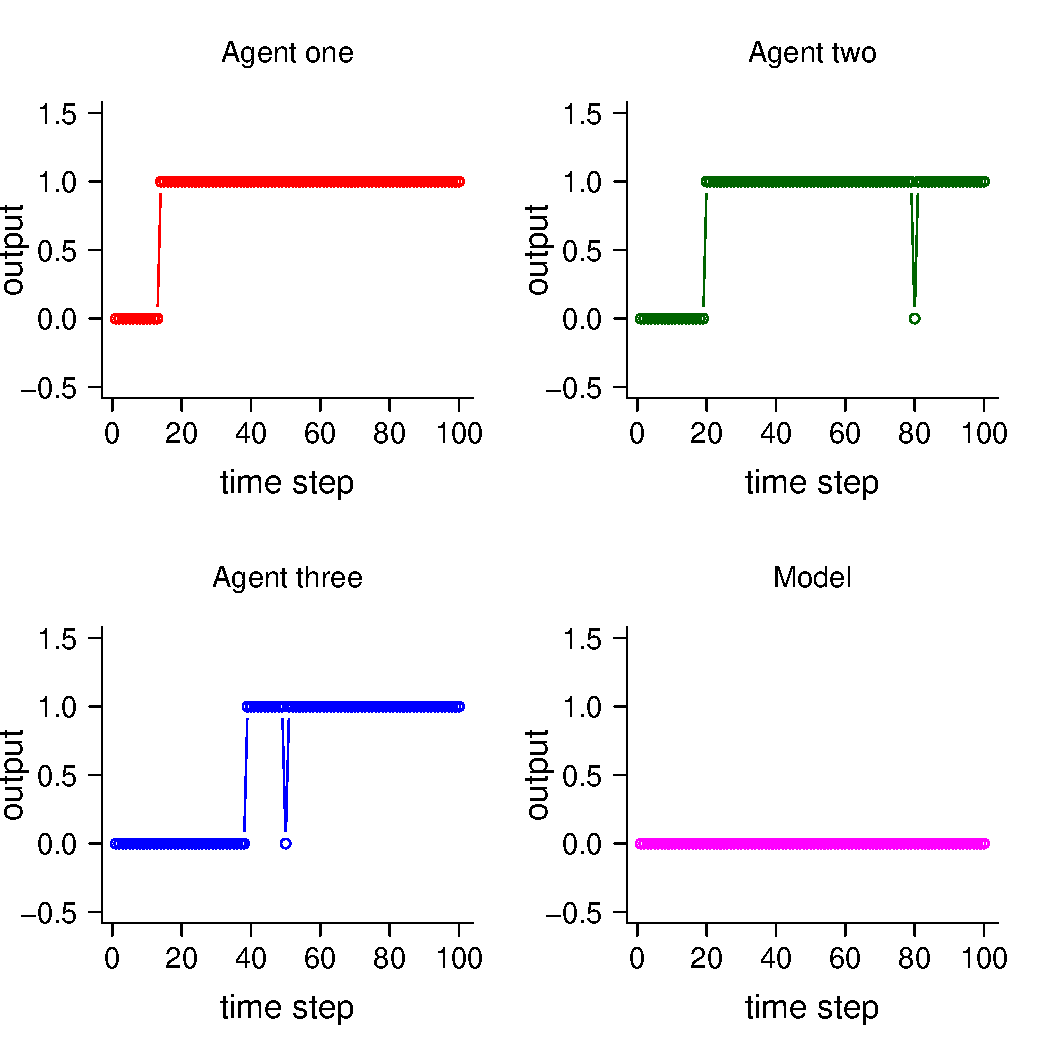
\includegraphics[width=3.0 in]{classifier_output_sequence.pdf}
		}\\
		\subfloat[(b) activation of hidden neurons\label{fig:classifier_output_hidden_neurons}]{%
			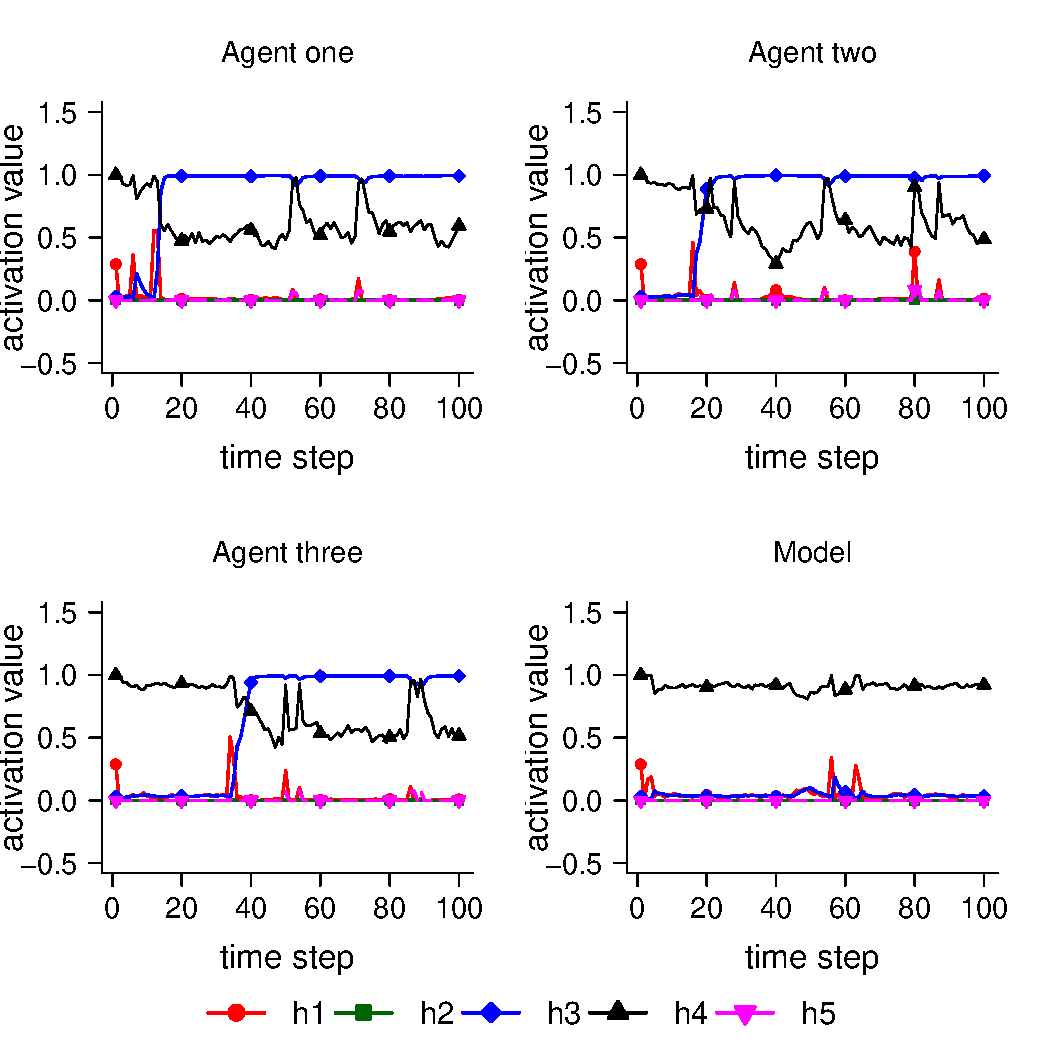
\includegraphics[width=3.0 in]{classifier_output_hidden_neurons.pdf}
		}
		\caption{This plot shows the (a) decision-making process and (b) the corresponding activation value of the $5$ hidden neurons of a classifier for three random-chosen agents and the replica that executes a very good model in a trial. Hidden neurons are labeled as $\textrm{h}1$, $\textrm{h}2$, $\textrm{h}3$, $\textrm{h}4$, and $\textrm{h}5$.}
		\label{fig:classifier_output}
\end{figure}
\subsubsection{Using a Single Classifier}

The average decision accuracy of the classifier with the highest subjective fitness in $30$ coevolution runs is shown in Fig.~\ref{fig:classifier_decision_accuracy_swarm_simulation} (\textit{best classifier (subjective)}). The accuracy combines the percentage of correct judgments about models ($50\%$ weight) with the percentage of correct judgments about agents ($50\%$ weight). The accuracy of the classifier increases in the first $5$ generations, then drops and fluctuates within range $62\%$--$80\%$.
%There is some fluctuation during the evolutionary process, but the accuracy is always at a low value over generations. 

An alternative strategy is to select the classifier that achieves the highest fitness when evaluated on the whole historical tracking data (not just those of the current generation). The decision accuracy of this classifier is also shown in Fig.~\ref{fig:classifier_decision_accuracy_swarm_simulation} (\textit{best classifier (archive)}). The trend is similar to that of \textit{best classifier (subjective)}. The accuracy increases in the first $10$ generations,  and then starts \emph{decaying}, dropping to around $65\%$ by the $1000^\textrm{th}$ generation. However, in the earlier generations, the accuracy of the \textit{best classifier (archive)} is higher than that of the \textit{best classifier (subjective)}. For a comparison, we also plot the highest decision accuracy that a single classifier achieves for each generation (\textit{best classifier (decision)}). Interestingly, the accuracy of the \textit{best classifier (decision)}, which is shown in  Fig.~\ref{fig:classifier_decision_accuracy_swarm_simulation} (black curve), increases almost monotonically, reaching a level above $95\%$. Note that to select the \textit{best classifier (decision)}, one needs to perform additional trials ($146410$ in this case).

At first sight, it is counter-intuitive that selecting the best classifier according to the historical data still leads to low decision accuracy. This phenomenon, however, can be explained when considering the model population. We have shown in the previous section (see especially Fig.~\subref*{fig:model_parameters_convergence_aggregation}) that the models converge rapidly at the beginning of the coevolutions. As a result, when classifiers are evaluated in later generations, the trials are likely to include models very similar to each other. Classifiers that become overspecialized to this small set of models (the ones dominating the later generations) have a higher chance of being selected in the post-evaluation. These classifiers may however have a low performance when evaluated across the entire model space.
%The selected classifiers thus become overspecialized to a small set of models: the ones dominating the later generations. 

To investigate whether the decision accuracy is a good measurement of the quality of the classifiers, we plot a figure showing the fitness of the best classifiers corresponding to Figure~\ref{fig:classifier_decision_accuracy_swarm_simulation}. The fitness is calculated based on the $14641$ models. In addition, we also plot the classifier with the highest fitness for comparison, which is termed as~\textit{best classifier (objective)}. The results are shown in Figure~\ref{fig:classifier_fitness_swarm_simulation}. As we can see, the trend of fitness curves show good correspondence to that of the decision accuracy in Figure~\ref{fig:classifier_decision_accuracy_swarm_simulation}, although there is still a small gap between the~\textit{best classifier (decision)} and~\textit{best classifier (objective)}. This means measuring the quality of classifiers according to decision accuracy is a reasonable choice.

In order to understand how the classifiers make judgment, we analyze the internal processing through monitoring the activation of hidden neurons. Figure~\ref{fig:classifier_output} shows the decision-making process and the corresponding activation value of the $5$ hidden neurons of the classifier with the highest decision accuracy in the last generation of a coevolution run for $3$ randomly-chosen agents and the replica in a trial. The model executed on the replica has a parameter set of $(-0.7, -1.0, 1.0, -0.9)$, which is very near to that of the agent in Equation~\eqref{eq:aggregation_optimal_controller}. As we can see in Figure~\subref*{fig:classifier_output_sequence}, for the agents, the classifier outputs $0$ at the beginning, and after a certain time period outputs $1$. This means the classifier needs some time to make the correct judgment. Note that for some time steps after it started to output $1$, it still outputs $0$, but this happens only occasionally. For the model, it always outputs $0$.  This phenomenon can be explained by the activation value of the hidden neurons of the classifier. The classifier's activation value of the hidden neurons (labeled as $\textrm{h}1$, $\textrm{h}2$, $\textrm{h}3$, $\textrm{h}4$, and $\textrm{h}5$ in Figure~\subref*{fig:classifier_output_hidden_neurons}) reveals how it processes the motion of different individuals\footnote{Note that the activation of hidden neurons may not be the same for all the classifiers due to the symmetry of neural networks, but the dynamics is similar.}. It seems that the decision-making (``sudden jump'' in Figure~\subref*{fig:classifier_output_sequence}) of the classifier is related with the variation of $\textrm{h}3$ and $\textrm{h}4$. Consider the classification of the agents for example, at the beginning, $\textrm{h}3$ has a very low value (which is almost $0$) and then after some time it starts to increase. The variation tendency of $\textrm{h}4$ is opposite.  Every time the classifier's judgment starts to jump from $0$ to $1$, the value of $\textrm{h}3$ starts to surpass that of $\textrm{h}4$. $\textrm{h}1$, $\textrm{h}2$ and $\textrm{h}5$ are almost not activated during the whole period, although sometimes the activation of $\textrm{h}2$ influences the judgment of the classifier. For instance, there are two peaks at about $50^\textrm{th}$ and $80^\textrm{th}$ time step in $\textrm{h}2$ for agent two and three, which correspond to a wrong judgment of the classifier (that is, it outputs $0$) at the same point. For the model, all the hidden neurons are almost not activated.


\subsubsection{Using a Classifier System}

The results of the previous section have shown that using a single classifier is not a good solution; although there may be a good classifier in each generation, it may take significant effort (trials with agents) to find it.

To address this problem, we propose the use of a classifier system, that is, a number of classifiers working in tandem to judge a given candidate. We choose the best $10$ classifiers\footnote{Note that the number of classifiers chosen to form the system here is not necessarily optimal. There is no guarantee that the individually best few classifiers will form the best \emph{system} when working in tandem. In principle, one could exhaustively search every possible combination of a given number of classifiers from the population. However, this is often infeasible---with our settings of choosing $10$ classifiers out of $100$, $1.73\times 10^{13}$ possibilities exist. We therefore propose the heuristic of choosing the individually best classifiers to form the system, and empirically show that this nevertheless yields good results.}. This is either the set of $10$ classifiers with the highest subjective fitness in the current generation or the set of classifiers that achieve the highest fitness when evaluated on the whole historical data. If one or more classifiers make a decision about the candidate as a model (i.e. not an agent), the system outputs a ``model'' decision. Otherwise, it outputs ``agent''.

The results of using a classifier system are shown in Fig.~\ref{fig:classifier_decision_accuracy_swarm_simulation} (green and magenta, respectively). The two systems exhibit significantly improved decision accuracy across all generations. After $1000$ generations, each system has a high accuracy of above $95\%$, on average. 
%It seems that the classifiers in the system are complementary when making decision. 
%In stark contrast to the case of using a single classifier, 
\begin{figure}[!t]
    \centering
    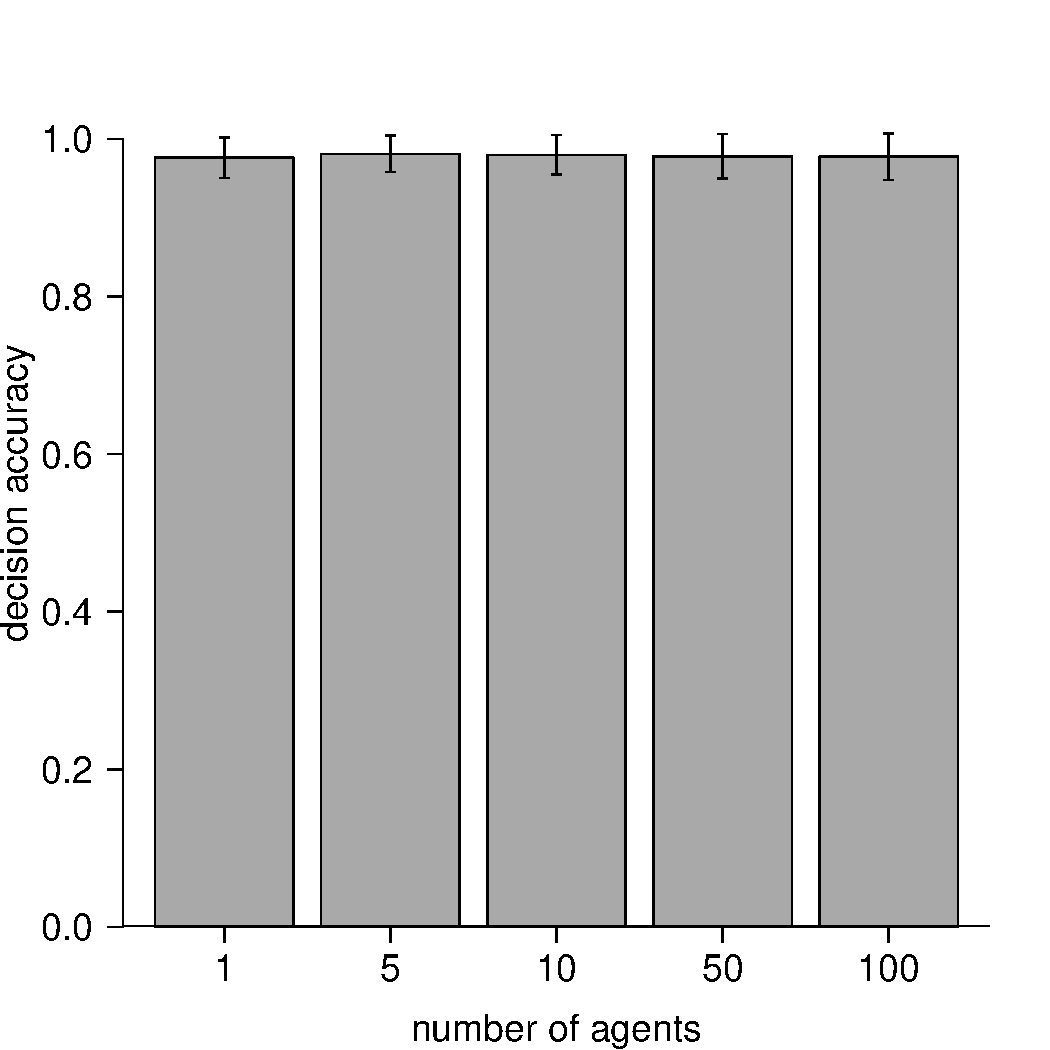
\includegraphics[width=3.5 in]{last_generation_classifier_scalability.pdf}
    \caption{This plot shows the decision accuracy of the~\textit{classifier system (archive)} in the $1000^\mathrm{th}$ generation of $30$ coevolution runs for different numbers of agents in the group. A single replica was present in each trial. In each case, $14641$ different models were tested.}
    \label{fig:classifier_scalability_aggregation}
\end{figure}
%
\begin{figure}[!t]%htbp
	\centering
	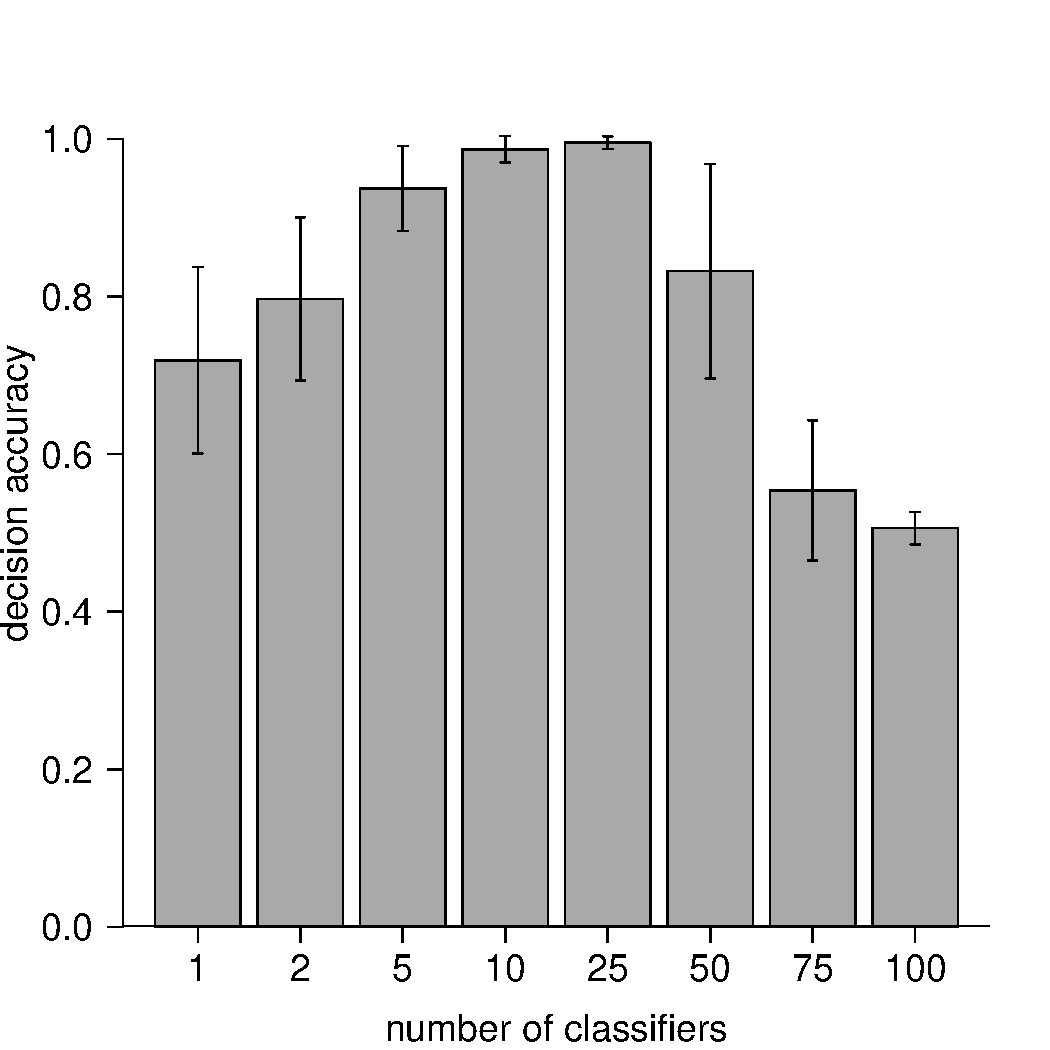
\includegraphics[width=3.5 in]{last_generation_judgment_accuracy_cf_num_selection.pdf}
	\caption{This plot shows the decision accuracy of the~\textit{classifier system (archive)} in the $1000^\mathrm{th}$ generation of $30$ coevolution runs with various number of classifiers chosen to form a system.}
	\label{fig:last_generation_judgment_accuracy_cf_num_selection}
\end{figure}

When post-evaluating the performance of classifier systems, we kept the setup the same as the one used in the coevolution runs (i.e., $10$ agents and $1$ replica in each trial). In practice, the ratio of agents and replicas in a trial could be different. Therefore, we analyzed the scalability of the classifier systems selected in the last generation over $30$ coevolution runs with different number of agents in the group. Note that there is always one replica in the group. We tested $14641$ different models. Figure~\ref{fig:classifier_scalability_aggregation} shows the decision accuracy of the~\textit{classifier system (archive)} when changing the number of agents in the group. As we can see, the decision accuracy of the classifier system is not affected by the variation of the number of agents, which shows the robustness of the classifier system.
%We have verified that with various number of replicas in the group, similar results are obtained.

As we mentioned before, we chose $10$ classifiers to form a classifier system to have a reasonable decision accuracy. Here we investigate how the classifier systems perform with various number of classifiers chosen to form a system. The decision accuracy of the~\textit{classifier system (archive)} is shown in Figure~\ref{fig:last_generation_judgment_accuracy_cf_num_selection}\footnote{The result of~\textit{classifier system (subjective)} is similar.}. It seems that as long as the number of classifiers chosen to form a system is within a certain range, the system could perform well. For example, when the number of selected classifiers is between $10$ and $25$, the classifier system can obtain a high decision accuracy. However, when the number is high (e.g., $75$), the decision accuracy declines dramatically.
%
\begin{figure}[!t]%htbp
	\centering
	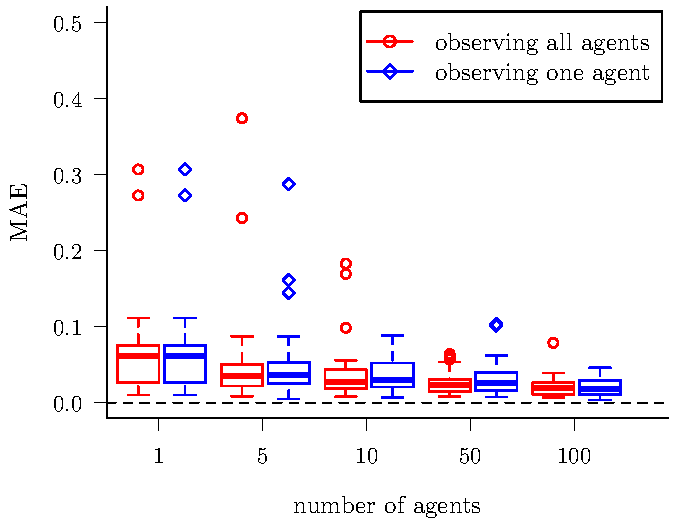
\includegraphics[width=3.5 in]{model_parameters_box_aggregation_scalability.pdf}
	\caption{MAE (defined in Equation~\eqref{eq:MAE}) of the evolved models with the highest subjective fitness after $1000$ generations, when using~\textit{Turing Learning} with varying numbers of agents (excluding the replica). Red and blue boxes show, respectively, the cases where all agents are observed, and one agent is observed. Boxes show distributions over $30$ coevolution runs. }
	\label{fig:model_parameters_box_aggregation_scalability}
\end{figure}
%
\subsection{Observing Only a Subset of Agents}\label{sec:observing_a_subset_agents_swarm_simulation}
So far, we have used motion data about all agents in the swarm when evaluating classifiers. However, this may not always be feasible in practice. For instance, given a video recording of a large and/or dense swarm, extracting motion data about all agents may be infeasible or lead to highly inaccurate results. A more practical solution might be to only track a subset of agents (e.g., by equipping them with markers).

We now compare the case where all agents are observed with the other extreme, where only one agent is observed. We study how these two cases compare as the swarm size increases. We conducted $30$ coevolution runs with each number of agents $n\in\left\{1, 5, 10, 50, 100\right\}$. There was always one replica in the group. When observing only one agent, this was chosen randomly in each trial. Note that the total number of trials in each coevolution run for the case of observing all agents and one agent is identical. We measured the total square error of the model with the highest subjective fitness in the last ($1000^\textrm{th}$) generation of each run. The results are shown in Fig.~\ref{fig:model_parameters_box_aggregation_scalability}.

There is no statistically significant difference for any $n$. On the other hand, as the swarm size increases, performance improves. For example, there is a statistically significant difference between $n=10$ and $n=100$, both when observing all agents and one. These results suggest that the key factor in the coevolutionary process is not the number of observed agents, so much as the richness of information that comes from increasing inter-agent interactions, and is reflected in each agent's motion. This means that in practice, observing a single agent is sufficient to infer accurate models, as long as the swarm size is sufficiently large.

A similar phenomenon was observed in a different scenario, where the goal was to distinguish between different `modes' of a swarm (i.e., global behaviors) through observing only a few individuals~\cite{Daniel2014}.

\begin{figure}[!t]%
	\centering
		\subfloat[(a) \label{fig:Angle_I=0}]{%
			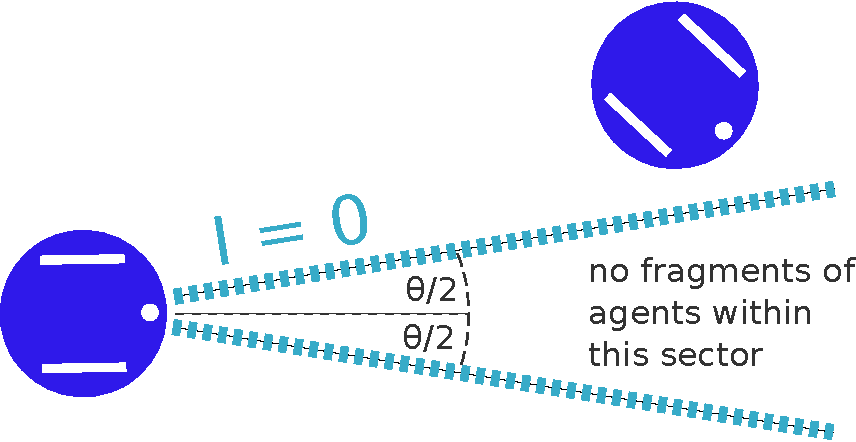
\includegraphics[width=2.2 in]{Angle_I=0.pdf}
		}\\
		\subfloat[(b) \label{fig:Angle_I=1}]{%
			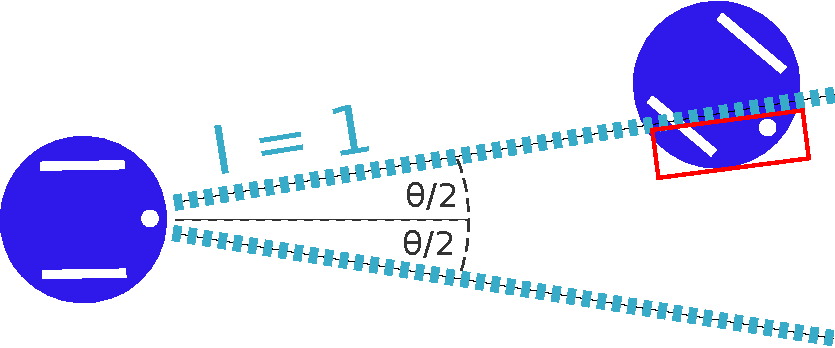
\includegraphics[width=2.2 in]{Angle_I=1.pdf}
		}
		\caption{A diagram showing the angle of view of the agent's sensor investigated in Section~\ref{sec:evolving_control_and_morphology_swarm_simulation}.}
		\label{fig:Angle_I}
\end{figure}

\begin{figure}[!t]%
	\centering
		\subfloat[(a) \label{fig:model_parameters_box_aggregation_0degree}]{%
			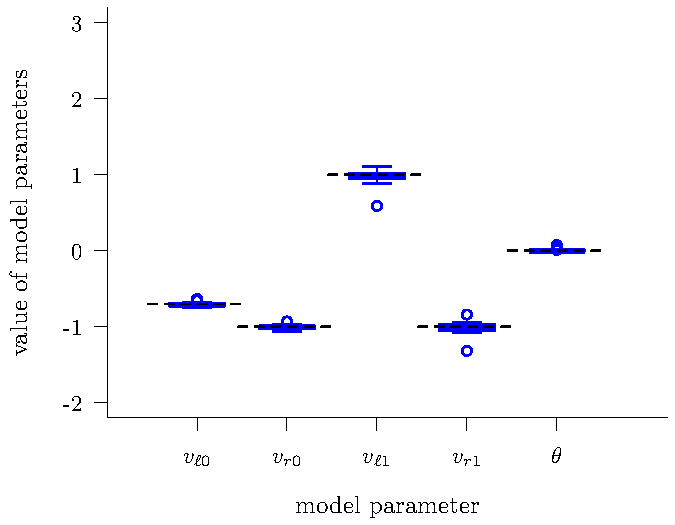
\includegraphics[width=3.5 in]{model_parameters_box_aggregation_0degree.pdf}
		}\\
		\subfloat[(b) \label{fig:model_parameters_box_aggregation_60degree}]{%
			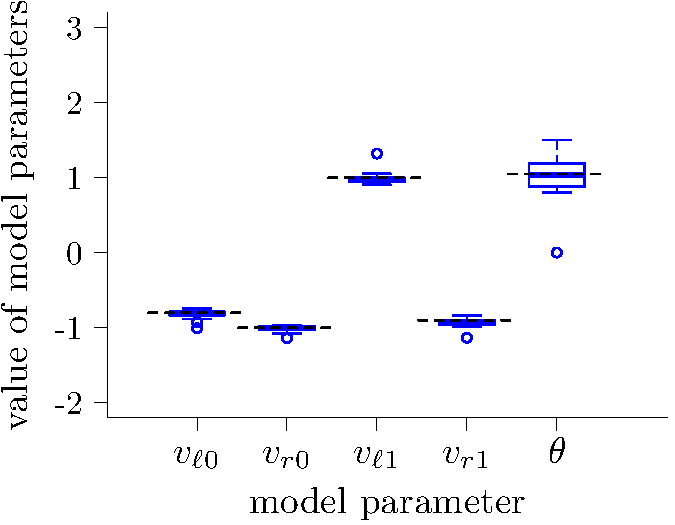
\includegraphics[width=3.5 in]{model_parameters_box_aggregation_60degree.pdf}
		}
		\caption{Parameters (controller parameters and angle of view in $\unit[]{rad}$) of the evolved models with the highest subjective fitness in the $1000^\textrm{th}$ generation corresponding to the case of the agents' angle of view equal to (a) $\unit[0]{rad}$ and (b) $\unit[\pi/3]{rad}$. Boxes show distributions over $30$ coevolution runs. Dotted black lines indicate true values.}
		\label{fig:model_parameters_box_aggregation_angle}
\end{figure}

\begin{figure}[!t]%
	\centering
		\subfloat[(a) \label{fig:model_parameters_convergence_aggregation_0degree}]{%
			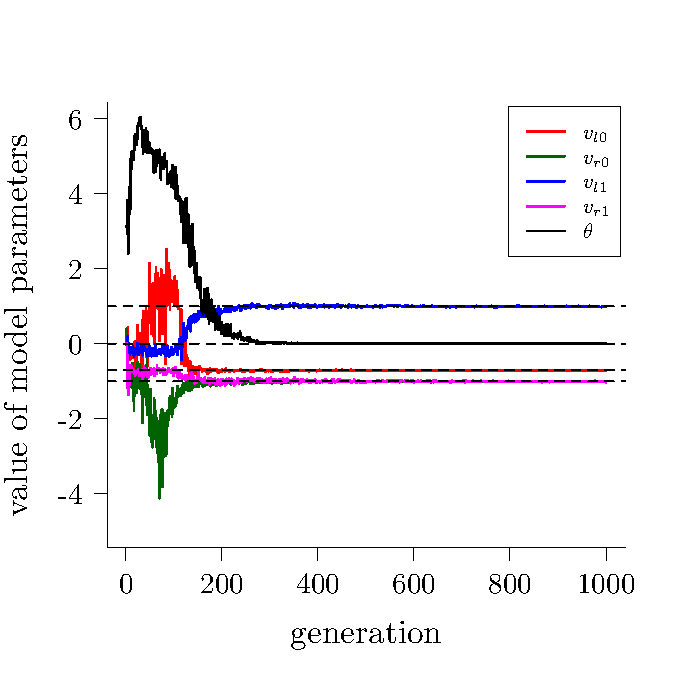
\includegraphics[width=3.5 in]{model_parameters_convergence_aggregation_0degree.pdf}
		}\\
		\subfloat[(b) \label{fig:model_parameters_convergence_aggregation_60degree}]{%
			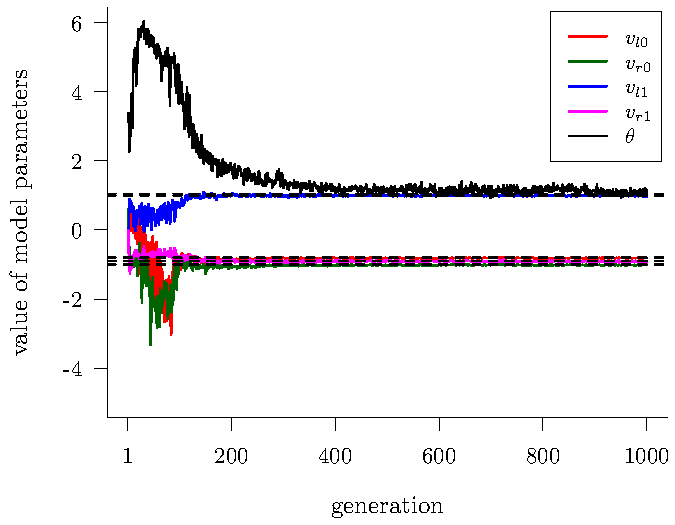
\includegraphics[width=3.5 in]{model_parameters_convergence_aggregation_60degree.pdf}
		}
		\caption{Evolutionary process of the evolved models (controller parameters and angle of view in $\unit[]{rad}$) in the $1000^\textrm{th}$ generation corresponding to the case of the agents' angle of view equal to (a) $\unit[0]{rad}$ and (b) $\unit[\pi/3]{rad}$. Boxes show distributions over $30$ coevolution runs. Dotted black lines indicate true values.. \label{fig:model_parameters_convergence_angleview}}
\end{figure}
%
\subsection{Evolving Control and Morphology}\label{sec:evolving_control_and_morphology_swarm_simulation}
In the previous sections, we assumed that we fully knew the agents' morphology (i.e., structure), and only their behavior (controller) was to be identified. We now present a variation where one aspect of the morphology is also unknown. The replica, in addition to the four controller parameters, takes a parameter $\theta\in\left[0,2\pi\right]\unit{rad}$, which determines the horizontal field of view of its sensor, as shown in Fig.~\ref{fig:Angle_I} (however, the sensor is still binary). Note that in the previous sections the agents' line-of-sight sensor can be considered as a sensor with angle of view of $\unit[0]{rad}$.

The models now have five parameters. As before, we let the coevolution run in an unbounded search space (i.e., now, $\mathbb{R}^5$). However, as $\theta$ is necessarily bounded, before a model was executed on a replica, the parameter corresponding to $\theta$ was mapped to the range $[0, 2\pi]$ using a logistic sigmoid function (Equation~\eqref{equ:logistic_sigmoid}). The controller parameters were directly passed to the replica. In this setup, the classifiers observed the individuals for $\unit[100]{s}$ in each trial (preliminary results indicated that this setup requires a longer observation time). 

Fig.~\subref*{fig:model_parameters_box_aggregation_0degree} shows the parameters of the subjectively best models in the last ($1000^\textrm{th}$) generations of $30$ coevolution runs. The means (standard deviations) of the AEs in each model parameter were: $0.02$ ($0.01$), $0.02$ ($0.02$), $0.05$ ($0.07$), $0.06$ ($0.06$) and $0.01$ ($0.01$). All parameters including $\theta$ were still learned with high accuracy.

The case where the true value of $\theta$ is $\unit[0]{rad}$ is an edge case, because given an arbitrarily small $\epsilon>0$, the logistic sigmoid function maps an infinite domain of values onto $(0,\epsilon]$. 
%(i.e., $\forall\epsilon>0.\, \exists x_0.\, \forall x<x_0.\, \textrm{sig}\,x < \epsilon $). 
This makes it easier for the coevolution to learn this parameter. For this reason, we also considered another scenario where the agents' angle of view is $\unit[\pi/3]{rad}$ rather than $\unit[0]{rad}$. The controller parameters for achieving aggregation in this case are different from those in Equation~\eqref{eq:aggregation_optimal_controller}. They were found by re-running a grid search with the modified sensor. Fig.~\subref*{fig:model_parameters_box_aggregation_60degree} shows the results from $30$ coevolutions with this setup. The means (standard deviations) of the AEs in each parameter were: $0.04$ ($0.04$), $0.03$ ($0.03$), $0.05$ ($0.06$), $0.05$ ($0.05$) and $0.20$ ($0.19$). The controller parameters were still learned with good accuracy. The accuracy in the angle of view is noticeably lower, but still reasonable.

\begin{figure}[!t]%
	\centering
		\subfloat[(a) \label{fig:MAE_histgram_random_controllers}]{%
			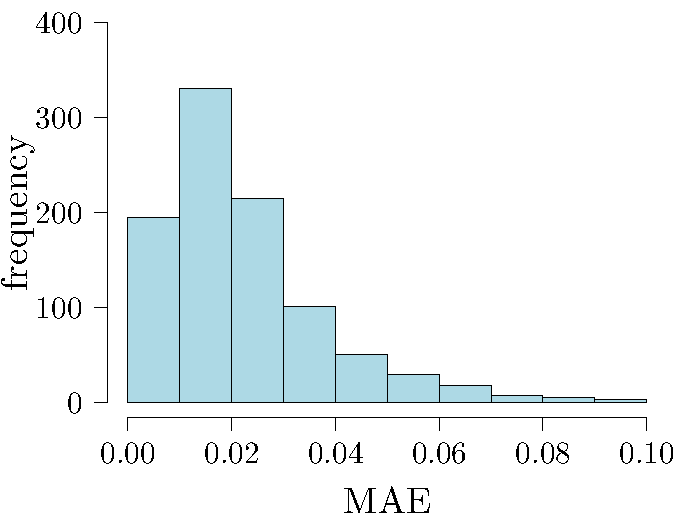
\includegraphics[width=3.5 in]{MAE_histgram_random_controllers.pdf}
		}\\
		\subfloat[(b) \label{fig:AE_box_random_controllers}]{%
			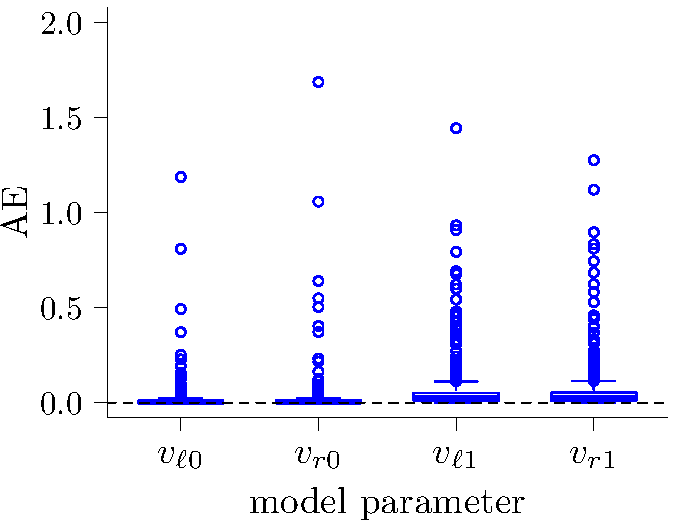
\includegraphics[width=3.5 in]{AE_box_random_controllers.pdf}
		}
		\caption{This plot shows (a) a histogram of the MAE (defined in Equation~\eqref{eq:MAE}) of the evolved models and (b) the AEs (defined in Equation~\eqref{eq:AE}) of each model parameter in the $1000^\textrm{th}$ generation over $1000$ random behaviors. For each behavior, we performed one coevolution run. In (a), $43$ points that have MAE larger than $0.1$ are not shown.}
		\label{fig:model_parameters_random_controllers}
\end{figure}

\subsection{Evolving Other Behaviors}\label{sec:evolving_other_behaviors_swarm_simulation}
The aggregation controller that agents used in our case study was originally synthesized by searching over the space $\left[-1,1\right]^4$, using a metric to assess the swarm's global performance~\cite{Gauci2014_ijrr}. Other points in this space lead to different global behaviors that can be `meaningful' to a human observer (e.g. circle formation~\cite{Melvin_DARS2014}). 
%However, many other controllers may not lead to `meaningful' global behaviors.

We now investigate whether our coevolutionary method can learn arbitrary controllers in this space, irrespective of the global behaviors they lead to. We generated $1000$ controllers randomly in $[-1,1]^4$, with uniform distribution. For each controller we performed one coevolution run, and selected the subjectively best model in the last ($1000^\textrm{th}$) generation. 

Fig.~\subref*{fig:MAE_histgram_random_controllers} shows a histogram of the MAE of the evolved models. The distribution has a single mode close to zero, and decays rapidly for increasing values. Over $89\%$ of the $1000$ cases have an error below $0.05$. This suggests that the accuracy of~\textit{Turing Learning} is not highly sensitive to the particular behavior under investigation (i.e., most behaviors are learned equally well). Fig.~\subref*{fig:AE_box_random_controllers} shows the AEs of each model parameter. The means (standard deviations) of the AEs in each parameter were: $0.01$ ($0.05$), $0.02$ ($0.07$), $0.07$ ($0.6$) and $0.05$ ($0.20$). We performed a statistical test on the AEs between the model parameters corresponding to $I=0$ ($v_{\ell0}$ and $v_{r0}$) and $I=1$ ($v_{\ell1}$ and $v_{r1}$). The AEs of the evolved $v_{\ell0}$ and  $v_{r0}$ were significantly lower than those of the evolved $v_{\ell1}$ and  $v_{r1}$. This was likely due to the reason reported in Section~\ref{sec:analysis_evolved_models_swarm_simulation}; that is, an agent spends more time seeing nothing ($I=0$) than other agents ($I=1$) in each trial.
\begin{figure}[!h]%htbp
	\centering
	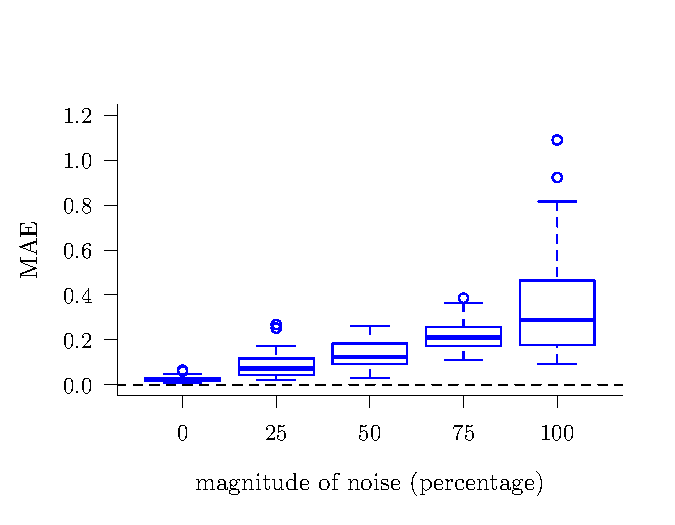
\includegraphics[width=3.5 in]{MAE_noise_study.pdf}
	\caption{This plot shows the MAE (defined in Equation~\eqref{eq:MAE}) of the evolved parameters when increasing the percentage of noise on the measurements of the individuals' position and orientation in the aggregation behavior. Each box corresponds to 30 coevolution runs. See text for details.
\label{fig:noise_study}}
\end{figure}

\subsection{Noise Study}\label{sec:noise_study_swarm_simulation}

We conducted a study to investigate how the performance of~\textit{Turing Learning} is affected by noise on the measurements of the individuals' position and orientation. As the e-puck robot has a maximum linear speed of $12.8\,\textrm{cm/s}$, the maximum distance that it can travel in one control cycle ($0.1\,\textrm{s}$) is $1.28\,\textrm{cm}$. For this reason, we define a disturbance of $1.28\,\textrm{cm}$ to an individual's position as a measurement error of $100\%$. Similarly, we define a $100\%$ measurement error on the individual's orientation as the maximum change in orientation that an e-puck can undergo in one control cycle. This corresponds to $0.5\,\textrm{rad}$.

We conducted $5$ sets of $30$ coevolutions for the noise values $M=\{0, 25, 50, 75, 100\}\%$. In a coevolution with a noise value $M$, every measurement of an individual's position is perturbed in a random direction and by a random distance chosen uniformly in $\left[0, 1.28\frac{M}{100}\right] \,\textrm{cm}$. Similarly, every orientation measurement is perturbed by a random angle chosen uniformly in $\left[-0.5\frac{M}{100}, 0.5\frac{M}{100}\right]$.

Figure~\ref{fig:noise_study} shows MAE (defined in Equation~\eqref{eq:MAE}) of the evolved parameters in the final generations of the coevolutions. This plot reveals that the system still performs relatively well when a considerable amount of noise affects the individuals' motion tracking system.

\section{Summary}\label{sec:summary_simulation_swarm}

This chapter has presented the simulation results of using the~\textit{Turing Learning} method to autonomously learn swarm behaviors through observation. To our knowledge, \textit{Turing Learning} is the first system identification method that does not rely on any predefined metric to quantitatively gauge the difference between agents and learned models. This eliminates the need to choose a suitable metric and the bias that such metric may have on the obtained solutions. 

Through competitive coevolution of models and classifiers, the system successfully learned two swarm behaviors (self-organized aggregation and object clustering). Both the model parameters, which were automatically inferred, and emergent global behaviors closely matched those of the original swarm system. We also constructed a robust classifier system that, given an individual's motion data, can tell whether the individual is an original agent or not. Such classifier system could be effective in detecting abnormal behavior, for example, when faults occur in some members of the swarm. Note that~\textit{Turing Learning} produces these classifiers automatically without the need to define a priori what constitutes abnormal behavior. 
%The performance of the classifier system was better than that of any single classifier, as the classifiers were found to collaborate in the coevolution. 

A scalability study showed that the interactions in a swarm can be characterized by the effects on a subset of agents. In other words, when learning swarm behaviors especially with large number of agents, instead of considering the motion of all the agents in the group, we could focus on a subset of agents. This becomes critical when the available data about agents in the swarm is limited. Our approach was proven to work even if using only the motion data of a single agent and replica, as the data from this agent implicitly contained enough information about the interactions in the swarm.   

In this chapter, the model was explicitly represented by a set of parameters. The evolved parameters could thus be compared against the ground truth, enabling us to objectively gauge the quality of evolved models in two case studies as well as for $1000$ randomly sampled behaviors. In principle, we could also evolve the structure of the agent's control system. The results of learning the agent's angle of view showed that our method may even learn the morphology of the swarming agents.
%However, this should not be considered as an inherent limitation of our method. , using an implicit representation (e.g. neural network)
%In the two case studies investigated, the behaviors of the agents in the group were almost not affected by inserting the replica in each trial. 

In collective behavior, abnormal agent(s) may have a great impact on the swarm~\cite{Bjerknes2013}. For the same reason, the insertion of a replica that exhibits different behavior or is not recognized as con-specific may disrupt the global behavior and hence the models obtained may be biased. An appropriate strategy would be to isolate the influence of the replica. In particular, to evaluate a model one could perform two trials, one with only replicas each executing the model and the other with only agents. The data of the replicas and agents from each trial could then be fed into the classifiers for making judgments. Some preliminary results suggest that there is no significant difference between either approach for the case studies considered in this chapter. In Chapter~\ref{ch:interaction}, we use~\textit{Turing Learning} to infer the behavior of a single agent. In all cases that are considered, either the agent or the replica is present. 



